\documentclass[a4paper,oneside,12pt]{book}
%----------------------------------------------------------------------------------------
%	WELCOME!
%   It's probably worth having a read through this file to set up the broad parameters.
%----------------------------------------------------------------------------------------

%----------------------------------------------------------------------------------------
%	COVER PAGE
%   The cover page is laid out in title/title.tex. You can choose a colour
%   or black and white logo
%----------------------------------------------------------------------------------------

%----------------------------------------------------------------------------------------
%	THESIS INFORMATION
%   Put title, author name, degree, type of work, school, department in here
%   It will be used for the title page and for the embedded PDF information
%----------------------------------------------------------------------------------------

\newcommand{\thesistitle}{Learning for sensor-based, real-time fall detection for cyclists.  } % Your thesis title, this is used in the title and abstract
\newcommand{\degree}{B. A (Mod.) Computer Science} % Your degree name, this is used in the title page and abstract
\newcommand{\typeofthesis}{Final Year Project} % dissertation, Final Year Project, report, etc.
\newcommand{\authorname}{Aidan Mongan} % Your name, this is used in the title page and PDF stuff
%% Comment out the next line if you don't want your ID to appear
\newcommand{\authorid}{14334583} % Your ID
\newcommand{\keywords}{this, that, more} % Keywords for your thesis
\newcommand{\school}{\href{http://www.scss.tcd.ie}{School of Computer Science and Statistics}} % Your school's name and URL, this is used in the title page

%% Comment out the next line if you don't want a department to appear
%\newcommand{\department}{\href{http://researchgroup.university.com}{Department Name}} % Your research group's name and URL, this is used in the title page

\AtBeginDocument{
\hypersetup{pdftitle=\thesistitle} % Set the PDF's title to your title
\hypersetup{pdfauthor=\authorname} % Set the PDF's author to your name
\hypersetup{pdfkeywords=\keywords} % Set the PDF's keywords to your keywords
\hypersetup{pdfsubject=\degree} % Set the PDF's keywords to your keywords
}

%% Language and font encodings
\usepackage[T1]{fontenc} 
\usepackage[utf8]{inputenc}
\usepackage[english]{babel}

%% Bibliographical stuff
\usepackage[round,sort,comma,numbers]{natbib}

%% Document size
% include showframe as an option if you want to see the boxes
\usepackage[a4paper,top=2.54cm,bottom=2.54cm,left=2.54cm,right=2.54cm,headheight=16pt]{geometry}

%% Useful packages
\usepackage{amsmath}
\usepackage[autostyle=true]{csquotes} % Required to generate language-dependent quotes in the bibliography
\usepackage[pdftex]{graphicx}
\usepackage[colorinlistoftodos]{todonotes}
\usepackage[colorlinks=true, allcolors=black]{hyperref}
\usepackage{caption} % if no caption, no colon
\usepackage{sfmath} %use sans-serif in the maths sections too
\usepackage[parfill]{parskip}    % Begin paragraphs with an empty line rather than an indent
\usepackage{setspace} % to permit one-and-a-half or double spacing
\usepackage{enumerate} % fancy enumerations like (i) (ii) or (a) (b) and suchlike
\usepackage{booktabs} % To thicken table lines
\usepackage{fancyhdr}
\usepackage{wrapfig}



\pagestyle{plain} % Embrace simplicity!

%% The Mechanical engineers require your name and ID on the top of every page.
%% Uncomment the following block if you want your name and ID at the top of
%% (almost) every page.

%\pagestyle{fancy}
%\fancyhf{} % sets both header and footer to nothing
%\renewcommand{\headrulewidth}{0pt}
%\cfoot{\thepage}
%\ifdefined\authorid
%\chead{\it \authorname\ (\authorid)}
%\else
%\chead{\it \authorname}
%\fi
%% End of block

%% It is not a requirement of the university that the font should be sans-serif, but
%% the Mechanical engineers require it. Comment out the following line to disable it
\renewcommand{\familydefault}{\sfdefault} %use the sans-serif font as default

%% If you're not using sans-serif, consider using Palatino instead of the LaTeX standard
%\usepackage{mathpazo} % Use the Palatino font by default if you prefer it to Computer Modern

\renewcommand{\theequation}{\arabic{equation}} %% use continuous equation numbers

%% Format Chapter headings appropriately
\usepackage{titlesec}
\titleformat{\chapter}[hang] 
{\normalfont\huge\bfseries}{\thechapter}{1cm}{} 

\title{\thesistitle}
\author{\authorname}

\frontmatter

\usepackage{listings}
\usepackage{color}


\definecolor{dkgreen}{rgb}{0,0.6,0}
\definecolor{gray}{rgb}{0.5,0.5,0.5}
\definecolor{mauve}{rgb}{0.58,0,0.82}









\begin{document}
\begin{titlepage}

\center % Center everything on the page

%% All the text parameters should be taken from the start of the main.tex file.
%% You should only alter stuff here if you want to change the layout

%----------------------------------------------------------------------------------------
%	LOGO SECTION
%----------------------------------------------------------------------------------------
%% Choose one of the following -- a colour or black-and-white logo


\includegraphics{title/Trinity_RGB_transparent_main.png}\\[1cm] 
%
\includegraphics[width=12cm]{title/black-stacked-trinity.jpg}\\[1cm] 

\Large \school\\[1.5cm] % Minor heading such as course title
\ifdefined\department
\large \department\\[1.5cm] % Minor heading such as course title
\fi

%----------------------------------------------------------------------------------------
%	TITLE SECTION
%----------------------------------------------------------------------------------------
\makeatletter
{ \huge \bfseries \thesistitle}\\[1.5cm] % Title of your document
 

%----------------------------------------------------------------------------------------
%	AUTHOR SECTION
%----------------------------------------------------------------------------------------

\ifdefined\authorid
\authorname\\ % Your name
\authorid\\[2cm] % Your Student ID
\else
\authorname\\[2cm] % Your name
\fi

%----------------------------------------------------------------------------------------
%	DATE SECTION
%----------------------------------------------------------------------------------------

{\large \today}\\[2cm] % Date, change the \today to a set date if you want to be precise

 
%----------------------------------------------------------------------------------------
%	TYPE OF THESIS SECTION
%----------------------------------------------------------------------------------------
 A \typeofthesis\ submitted in partial fulfilment\\of the requirements for the degree of\\
\degree

\vfill % Fill the rest of the page with whitespace

\end{titlepage}
\pagenumbering{roman}
\section*{\Huge{Declaration}}
\vspace{1cm}
I hereby declare that this project is entirely my own work and that it has not been submitted as an exercise for a degree at this or any other university.

\vspace{1cm}
I have read and I understand the plagiarism provisions in the General Regulations of the University Calendar for the current year, found at \url{http://www.tcd.ie/calendar}.
\vspace{1cm}

I have also completed the Online Tutorial on avoiding plagiarism `Ready Steady Write', located at
\url{http://tcd-ie.libguides.com/plagiarism/ready-steady-write}.
\vspace{3cm}

Signed:~\rule{5cm}{0.3pt}\hfill Date:~\rule{5cm}{0.3pt}

\chapter*{Abstract}
Like all extreme sports, mountain biking comes with the potential for serious injury to the rider in the event of an accident. Non fatal injuries can easily become fatal, when one is alone, far from help and potentially incapacitated. A study conducted by Paracelsus Medical University recorded injury rates as high as 16.8 injuries per 1000 hours of riding, with 22 being moderate and 16 being severe, with rider error being the leading cause \cite{studyOfMTBInjuries}. An automated crash detection system has the potential to be life saving in the worst of circumstances.

Existing discipline-specific solutions e.g., for road only or for mountain use only, on both hardware (Specialized’s AnGi) and software (Strava Beacon,Garmin) have inflexible detection algorithms focusing on using thresholds for only one to two data points. For example AnGi records values from its inbuilt gyroscope and accelerometer, while Garmin’s system uses only accelerometer values. Such threshold-based solutions pose issues in terms of high false detection rates and a single threshold value is unlikely to be suitable for different users at different skill levels.
  
 This project expands on previous research done in the area of wearable fall detection devices for the elderly, focusing on the design of a software solution for real-time fall detection. Three data points are used: raw sensor data from both a tri-axial gyroscope and a tri-axial accelerometer as well as the rate of change of speed, calculated via GPS. The proposed system utilizes learning techniques to improve detection rates and over time generates a more personalized model. Based on pre-captured training data of both regular riding and crashes, data is classified using a multivariable logistic regression model in real-time to determine whether a crash has occurred. Raw sensor data is captured from the inbuilt sensors present on android smartphones.

This approach is implemented as an android application called “RideSafe” and was evaluated using a user study, comprising of 16 participants at local trail centres over a 2 day period. Crash data was also collected, by means of intentional crashes in a controlled environment  for verification.  Results show that this system can successfully detect upwards of 80\% of crashes with a low rate of 18\% false positives.


\newpage
\onehalfspacing\raggedright %\raggedright turns off justification and hypenation

\section*{\Huge{Acknowledgements}}

I would like to thank my supervisor Siobhan, for her continuous support over the past 6 months.
My sincere gratitude to both family and friends for their invaluable advice and support received over the past 5 years.
I also wish to thank my tutor Dr. Hugh Gibbons, without whom, I may not have made it through to my final year.
Finally a special thanks to everyone who partook in this study, especially Matt from Glencullen Adventure Park for allowing testing to take place on site.


\tableofcontents
\listoffigures
\listoftables
\lstlistoflistings
\newpage


\mainmatter
\chapter{Introduction}

\section{Motivation }

Personal experiences were the main driving factor in my motivation to pursue this study. As a mountain biker with 10 years of experience I have sustained my fair share of minor injuries, but witnessing injuries sustained by more venerable fellow riders are sometimes more impactful. Last summer on a seemingly normal spin with a friend, we discovered a woman lying injured off on the trail side, incapacitated and unable to call for help so I did on her behalf. Multiple phone calls later to aid the first responders in locating us they arrived - around 1 hour after impact.  This experience made me realize how useless your mobile phone is to you in these situations when one is unable to even pick it up.

Currently there are 29,000 registered members of cycling Ireland and with mountain biking  becoming ever more popular each year this number is set to grow. 


\section{Aims}


The  aim of this project was to develop an android application for real-time fall detection for cyclists,  automating the process of requesting assistance, and to reduce response time in the event of an accident. Before development of the application I set myself strict aims to achieve. 

\subsection*{Simplistic and Intuiative}
After the initial set up process, to carry out the main use case: crash detection would be started and stopped with a single press of a button. Start the service, put your phone in your pocket and enjoy your time on you bike with piece of mind. Simple and convenient to use, removing the possibility of confusion for the end user, as the end users will be members of  the general public.
A simple user interface is important as the setting to which the app would be outdoors in potentially harsh weather conditions, external factors such as glare from the sun  and the possibility of moisture on the screen make high detailed, small user interface elements unsuitable. Less is more in this scenario.

\subsection*{Diverse}
Many existing systems are discipline specific, only working for one aspect of cycling i.e., for cross country usage only. I intend this app to have the potential to work for all disciplines of cycling. Targeting single disciplines would drastically reduce the number of potential users as well as producing highly undesirable, inaccurate results if used for the incorrect discipline.

\subsection*{Standalone}
Utilizing android smartphones built in sensors removes the need for extraneous external equipment for ride monitoring.  I intend the app to work as expected with one's phone placed in their pocket or bag, requiring no extra mounting equipment for either the rider or the bike.

\subsection*{Enjoyable user experience}
Many existing solutions exhibit deal breaking issues which ultimately causes the end user to stop using the system, I aim to eradicate the pitfalls present in other systems leading to a better user experience. 

\subsection*{Efficiency}
Performance in terms of battery usage is of utmost importance, heavy battery usage would have the potential to kill the phone when one would need it most - in an emergency. Every possible optimization in terms of battery will be made where possible - without impacting performance.

\section{Personal Goals}
In addition to the aims of this project I had set some personal goals to achieve from undertaking this project.

\subsection*{Devolop a fully functional application.}
Having had brief experience working with android studio before undertaking this project to develop simple applications, most of which were interfaces for arduino circuits connected via bluetooth, I had never developed such a large scale complex application prior to this project. I was excited to broaden my skill set and develop an application ready to be published to the google play store. 

\subsection*{Work with Embedded sensors.}
Having experience working with microcontrollers and various sensors, I was excited to utilize the plethora of available sensors present in android smartphones today. 

\subsection*{Collect and Analyse Real World Data.}
Datasets for what a bike accident looks like in terms of sensor values are few and far between, I was excited to conduct my own research with many unknowns to which I would need to discover. Having very few similar documented studies available I was very interested to study this particular system in the domain of cycling.  

\subsection*{Real world testing.}
I was aware before undertaking this study that it would involve a lot of real world data collection, analysis and testing. Being a crash detection application testing could not be simulated sitting at a desk, which meant all my testing would need to be done in the real world which proved both challenging and exciting.


\section{Readers Guide}
\subsection* {2 - Background}
This section will discuss the concept of fall/accident detection, exploring both the sport and medical applications. The two main approaches of fall detection will be discussed and the strong points as well as issues with each type of system will be discussed.

\subsection* {3 - Design}

here about design 

\subsection* {4 - Implementation}
here about implementation

\subsection* {5 - Evaluation}

evaluation goes here 

\subsection* {6 - Conclusion}

da CONCLUSION



\chapter{Background}
here is the background

\section{The Concept}

what fall detection is all about 

\section{Exsisting Solutions - Medical}

much work has been done .....

\subsection{Vision Based Approaches}
expensive 
privacy issues

\subsection{Sensor Based Approaches}

\section{Exsisting Solutions - Cycling}

\subsection{Garmin}

\subsection{Specilized's ANGI}

\section{Threshold based solutions}

\section {Supervised Machine Learning}

\chapter{System Design}



\section{Requirements}


\subsection{Functional Requirements}
\begin{itemize}
\item An accurate method of detecting incidents which may occur while cycling.
\item A more personalized detector, allowing better detection for riders of all abilities. 
\item As lightweight and efficient application as possible to enable compatibility with as many devices as possible, as well as reducing battery usage. 
\item Automatic SMS functionality to allow one to be located in the event of an accident.
\item Locate the rider accurately in the event of an accident as quickly as possible. 
\end{itemize}


\subsection{Non-Functional Requirements}
\begin{itemize}
\item Useful statistics computed and displayed for the user (Average Speed, Distance Travelled)
\item Google Map integration providing an accident heatmap to warn of potential dangers as well as plotting journeys.
\item A compass to help with navigation if both gps and internet connectivity are unavailable.
\end{itemize}


\newpage


\section{Interface Design}


%%%%%%%%%%%%%%%%%%%%%%%%%%%%%%%%%%%%%%%%
\begin{wrapfigure}{r}{0.5\textwidth}
\begin{center}
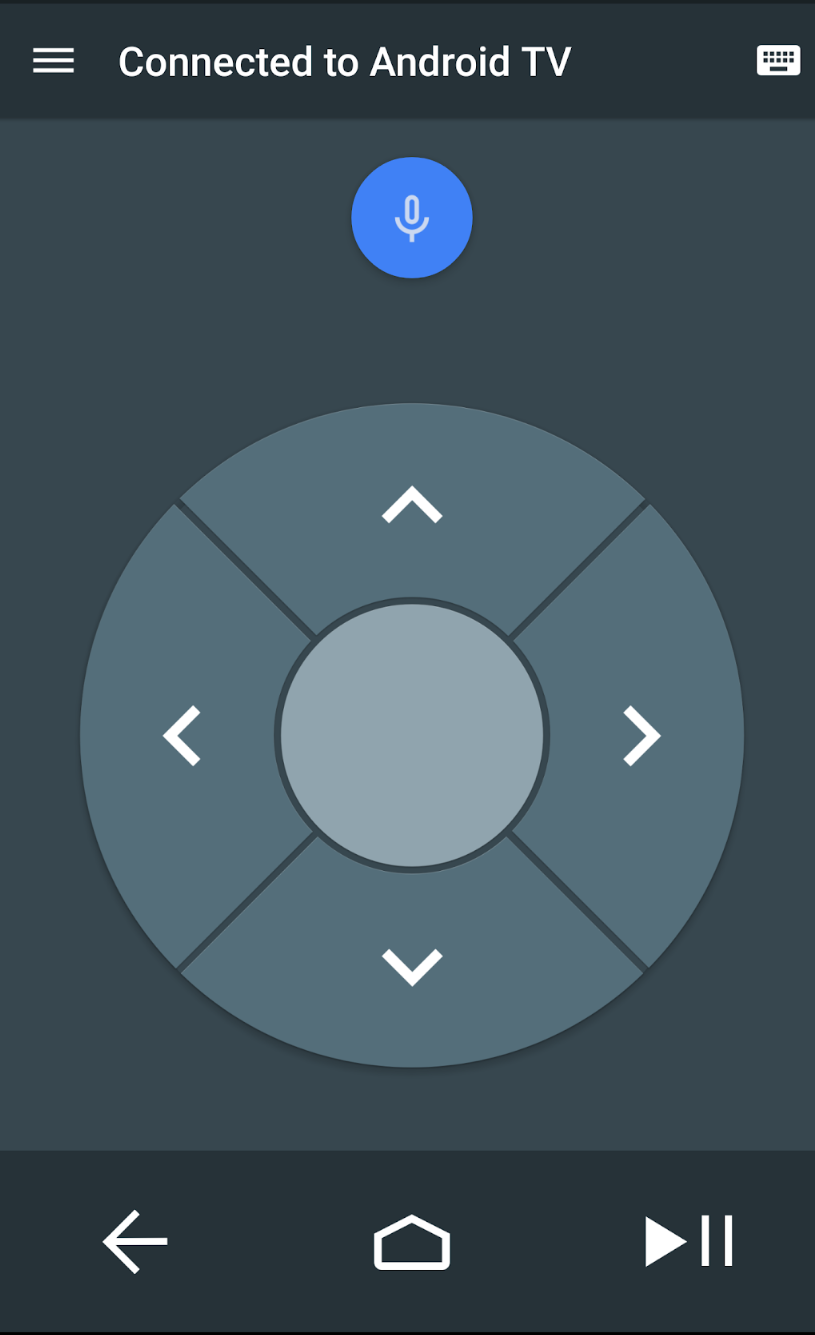
\includegraphics[scale = 0.4] {design/hs1.png}
\end{center}
\caption{Simple Home Screen Layout}
\label{hs1}
\end{wrapfigure}
%%%%%%%%%%%%%%%%%%%%%%%%%%%%%%%%%%%%%%%%

As simplicity and usability were key in the development of this application, the design of RideSafe was heavily influenced by Google's standard layout recommendations. For RideSafe functional requirements had a higher precedence than a fancy looking user interface. Inspiration was drawn from popular apps utility applications. As shown in figure \ref{hs1}  the main function of the application is the first screen the user will land on, removing extraneous steps required for the user to reach their goal - in this case change the channel. A simple uncluttered layout with only the necessary buttons required on the screen. 


%%%%%%%%%%%%%%%%%%%%%%%%%%%%%%%%%%%%%%%%
\begin{wrapfigure}{l}{0.5\textwidth}
\begin{center}
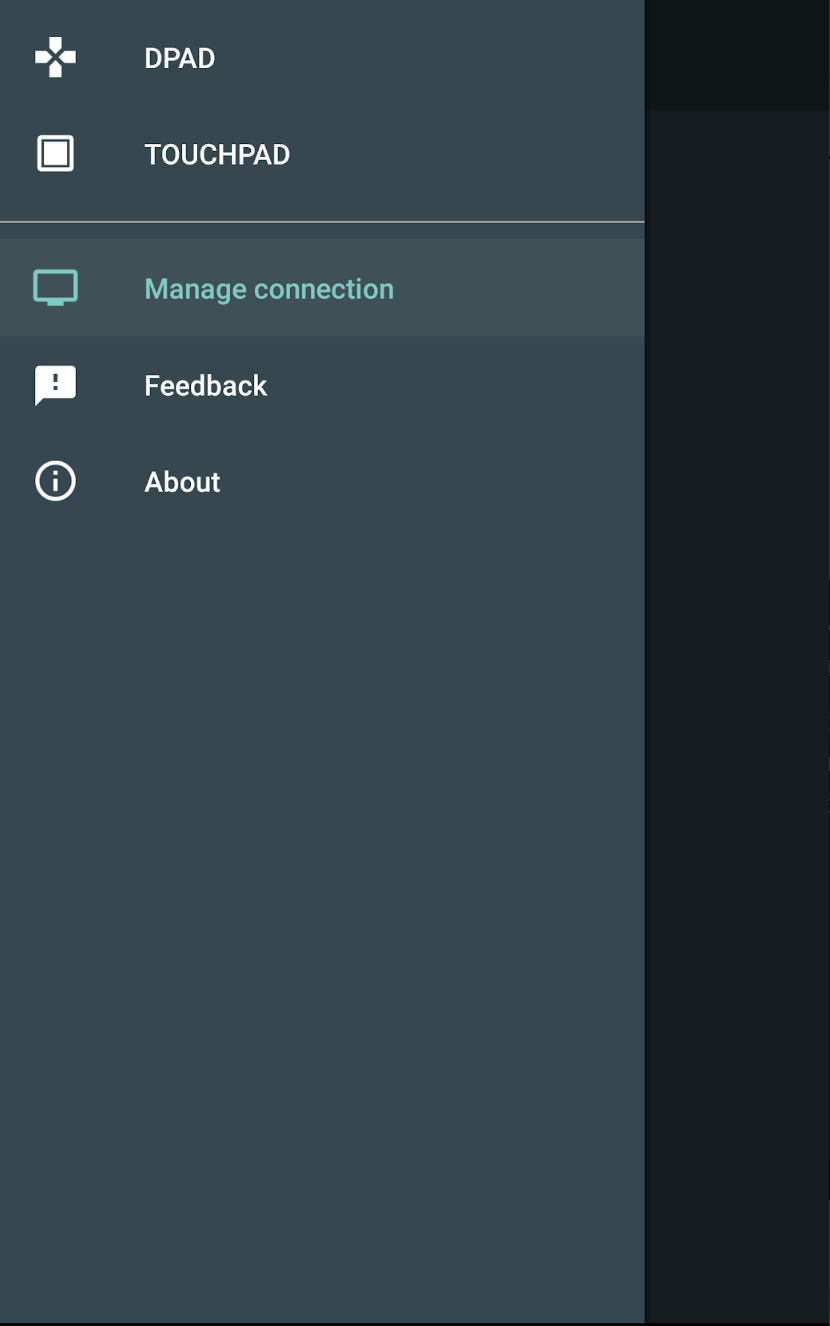
\includegraphics[scale = 0.4] {design/hme.png}
\end{center}
\caption{An Example implementation of A Navigation Drawer}
\label{hme}
\end{wrapfigure}
%%%%%%%%%%%%%%%%%%%%%%%%%%%%%%%%%%%%%%%%




For features less often used, Google's navigation drawer AKA the hamburger menu is a popular choice. As shown in figure \ref{hme} they are simple to use and allow for easy navigation to secondary functions of the application. Implementing a navigation drawer minimizes wasted space which would be taken up by adding a button for every secondary feature on the home screen, allowing the most important functionality to use up more screen real estate. As the hamburger menu is so common in every category of application on the play store, there is a high probability users will have encountered it before - resulting in a smaller learning curve to navigate through the application.


%%%%%%%%%%%%%%%%%%%%%%%%%%%%%%%%%%%%%%%%
\begin{wrapfigure}{c}{0.5\textwidth}
\begin{center}

\includegraphics[scale = .5] {design/logo.png}
\end{center}
\caption{App icon Inspiration}
\label{logo}
\end{wrapfigure}
%%%%%%%%%%%%%%%%%%%%%%%%%%%%%%%%%%%%%%%%


Colour and contrast of screen elements were a simple choice, having experience using my phone trailside in all conditions ranging from sweltering hot days to snowstorms. Simplicity is of utmost importance, glare on the screen makes any app impossible to see, especially apps featuring a dark theme.  My experience led me to favour a bright white theme with dark icons for maximum contrast. Accent colors were also an easy choice,  red was chosen as it is the color associated with “emergencies”  and “hospitals” figure \ref{logo}. Complementary shades of red were chosen using a material design palette generator \cite{color}.





\section{System Architecture Design}

This section will discuss in detail the method used to implement the crash detection logic used in RideSafe



\subsection{System Type}

Examining the vast amount of research done on fall detection in the medical domain, implementations which are threshold based could immediately be ruled out, as discussed in (section 2) threshold based solutions pose multiple issues in multiple areas, leading to the author not considering using this method.

A rule based implementation, with their proven accuracy and reliability was ultimately chosen to be the underlying architecture of ridesafe. Implementing a rule based system allows for more context to be considered measuring different data points at separate time frames, allowing the decision process to be based off a time interval rather than one moment in time. As will be discussed in the following subsection the author's choice of data points require a short period of time to determine if a crash has occurred rather than a single moment in time leading to a rule based solution to be the optimal solution.     


\subsection{Sensors \& Measurements}


Rather than just using the same data points used in existing solutions, the author launched an investigation into the suitability of different data points to determine if an accident has occurred. RideSafe Data Collection as it is now called is a logging application which was developed by the author to record multiple data points in multiple formats. While using the data collection application mountain biking over a period of a month at local trail centres. With a dataset containing tens of thousands lines of data points collected the data was visualized  and analized. For RideSafe my findings of the most relevant data points and sensors to utilize were chosen. 
\vspace{1cm}
\begin{itemize}
\item Triaxial Accelerometer
\end{itemize}


%%%%%%%%%%%%%%%%%%%%%%%%%%%%%%%%%%%%%%%%
\begin{wrapfigure}{r}{0.3\textwidth}
\begin{center}
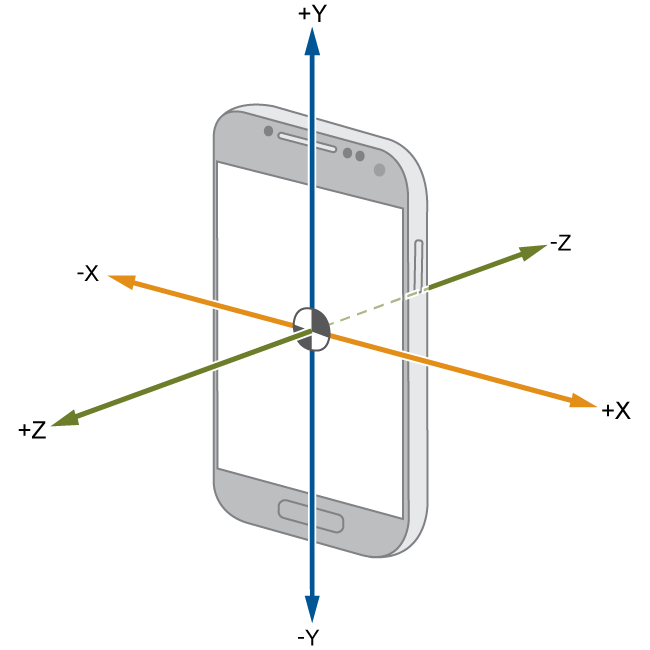
\includegraphics[scale = .2] {design/a.png}
\end{center}
\caption{Different Axis of an Accelerometer (Source Mathworks)}
\label{accel}
\end{wrapfigure}
%%%%%%%%%%%%%%%%%%%%%%%%%%%%%%%%%%%%%%%%

Like virtually every crash/fall detection solution, the triaxial accelerometer measuring linear acceleration of a body in three different axis as shown in figure \ref{accel} in \(m/s^2\). From my research the accelerometer was found to be a key sensor in determining if a crash has occurred. Using the well known Pythagorean theorem:  

\[
\mathit{} = 
\sqrt{x^2 + y^2 + z^2}
\]


  and accounting for the force of gravity on earth by subtracting  9.8 \(m/s^2\), directionless  g-force can be calculated. As the phones intended orientation is purposely unspecified directionless gforce is used to not require a certain axis to require a certain orientation.

\vspace{1cm}

\begin{itemize}
\item Triaxial Gyroscope
\end{itemize}

%%%%%%%%%%%%%%%%%%%%%%%%%%%%%%%%%%%%%%%%
\begin{wrapfigure}{l}{0.3\textwidth}
\begin{center}
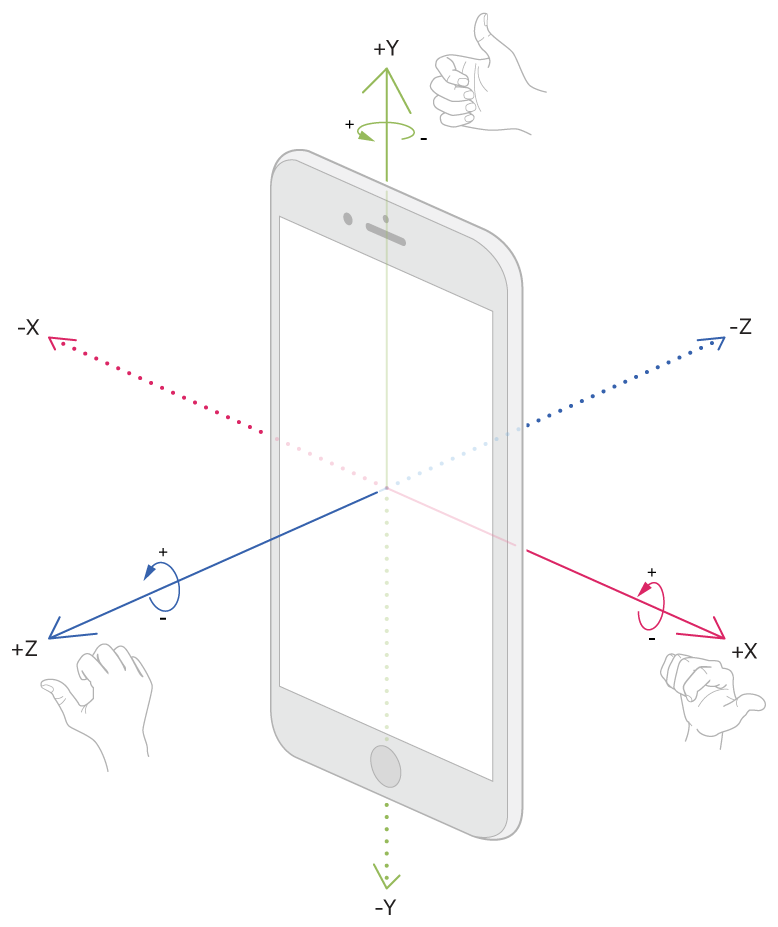
\includegraphics[scale = .1] {design/g.png}
\end{center}
\caption{Different Axis of a Gyroscope (Source Mathworks)}
\label{gyro}
\end{wrapfigure}
%%%%%%%%%%%%%%%%%%%%%%%%%%%%%%%%%%%%%%%%


The use of android's built in gyroscope allows for measuring rotational acceleration in three different axes as shown in figure \ref{gyro}. To measure rotational force in a certain direction the phone's orientation must be known, in this case where the orientation is unspecified total change in rotational acceleration was chosen, measuring the change in total rotation rather than on a per axis basis. The difference of the combined change in rotational acceleration is what the author found to be the most suitable reading. 
\vspace{1cm}

\begin{itemize}
\item Speed - GPS
\end{itemize}

From the authors investigation the change of speed was of great importance as a datapoint to consider. Many existing solutions for cycling re-use the logic found in fall detection for the elderly, a system designed to work indoor where speed isn't much of a factor. The author found that change of speed was directly related to a crash occurring as well as other activities. 

\vspace{2cm}
%%%%%%%%%%%%%%%%%%%%%%%%%%%%%%%%%%%%%%%%
\begin{figure}[h]
	\centering
	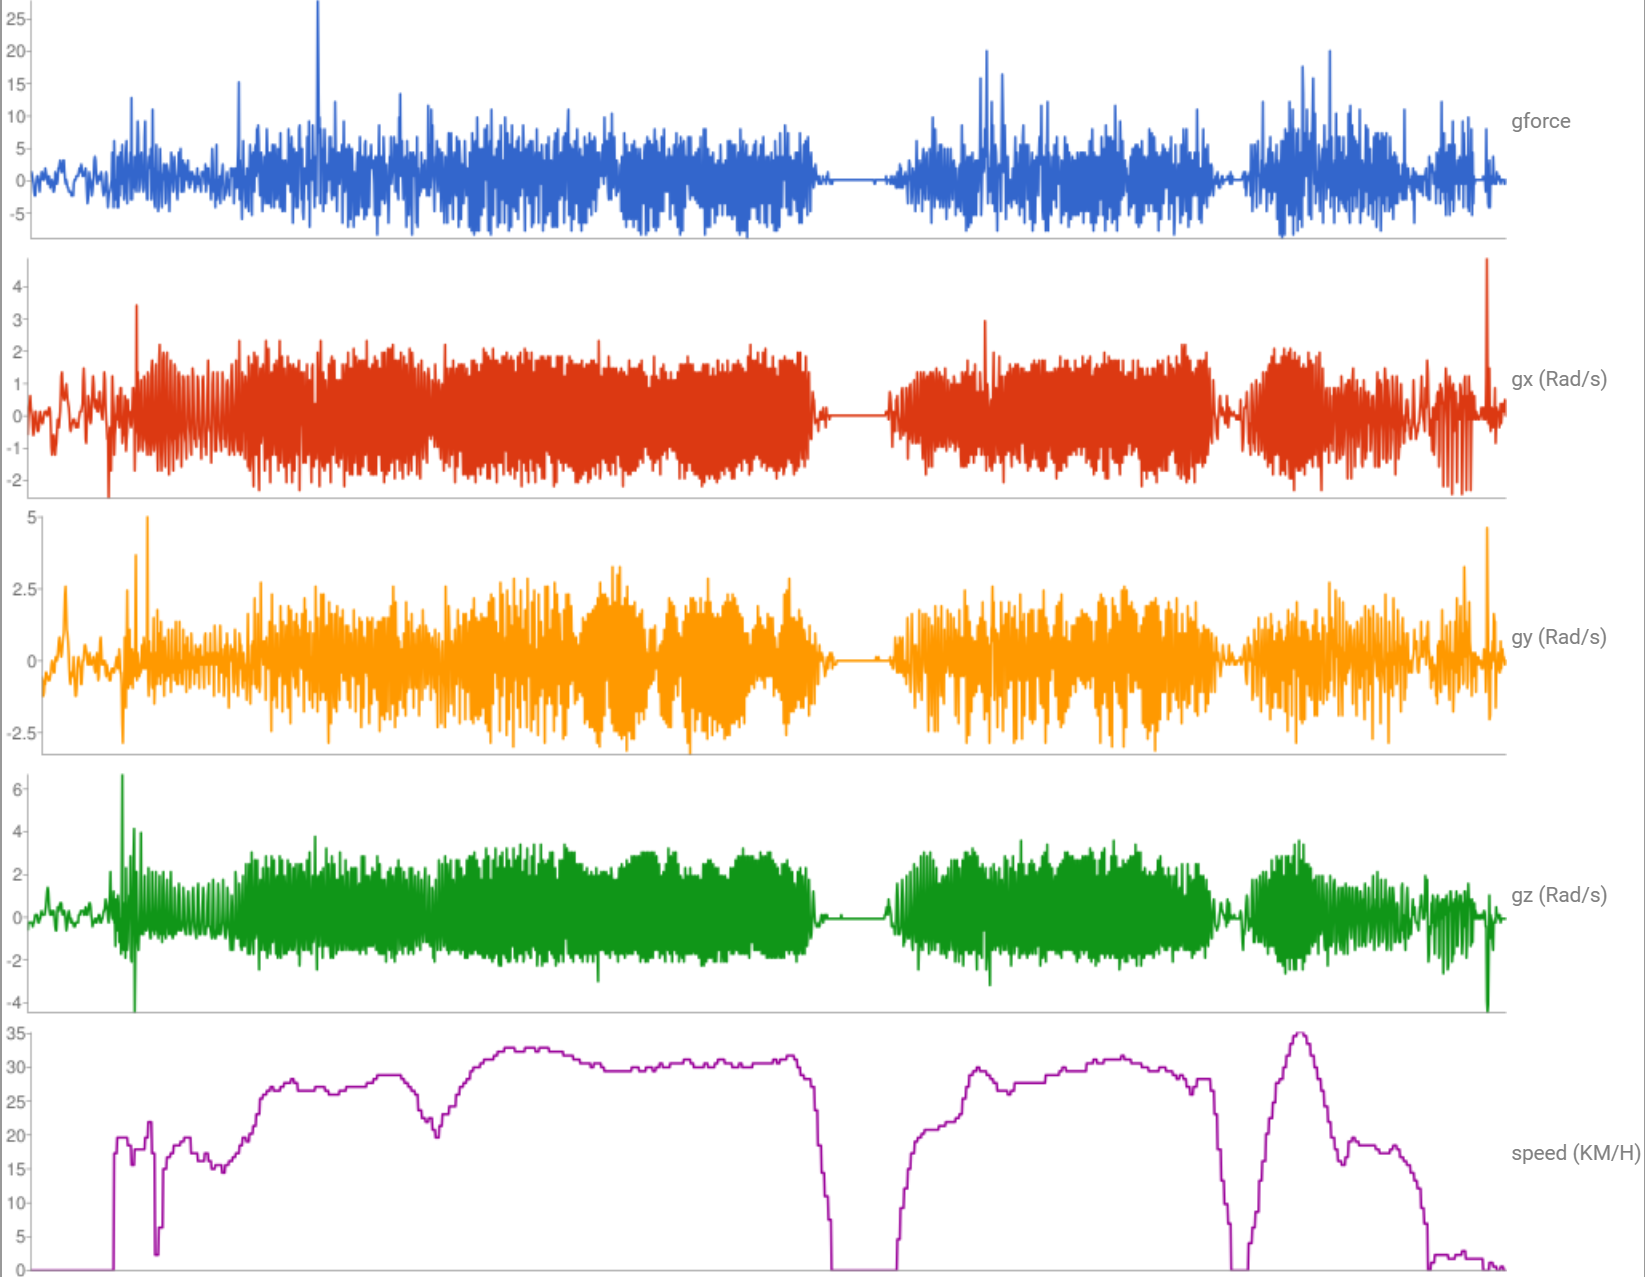
\includegraphics[scale = .7] {design/sampledata.png}
	\caption{G-Force, Angular Velocity and Speed  over time}
	\label{sampledata}
\end{figure}
%%%%%%%%%%%%%%%%%%%%%%%%%%%%%%%%%%%%%%%%
\vspace{1cm}

Figure \ref{sampledata} shows data collected from RideSafe data collection during a cycle in the Dublin mountains. The data represents a normal mountain bike spin on metro 1, spikes of g-force can be observed, as a result of landing jumps or simply a rough section of the trail. The large decreases in speed throughout the data are a result of extremely tight corners and or quick rests in between.

\newpage

\section{Machine Learning}



With this design we have multiple continuous variables to consider to determine if a crash has occurred.  Given the multiple current data values a probability needs to be computed. Using supervised machine learning outcome predictions can be made for given values once the model is trained with sufficient examples of both positive and negative examples. Researching commonly used machine learning techniques used in fall detection \cite{commonSolutions}, the author considered two possible methods. 
\begin{itemize}
\item Support vector machines (SVM)
\item Logistic Regression(LR)
\end{itemize}
Both SVM and (LR) are algorithms commonly used for classification, both performing comparably in practice. The main goal of both (LR) \& (SVM) are to calculate the best fitting line of divide in a given dataset, allowing for predictions to be made using similar data. SVM’s maximize the “line” of fit using support vectors maximizing the margin producing a class divide, outputting  a binary value 1 or 0 depending on class membership. LR using a sigmoid function outputs probabilities of a value belonging to class 1 between 0 and 1. LR allows for a manual class divide line to be set enabling a desired probability to set for the class divide. Logistic Regression's accuracy has been previously evaluated with both balanced and imbalanced data leading to accuracy exceeding 90\% in both cases \cite{suit}. Having previously studied Logistic regression paired with promising accuracy with test values, the author decided on basing the implementation on Logistic Regression due to the flexibility of the algorithm as well its simplicity to implement in java.



























\chapter{Implementation}
This chapter is split into three main sections:


\begin{itemize}
\item Technologies Used
\end{itemize}

Both the software and hardware used in the development for both RideSafe \& the companion data collection variant.



\begin{itemize}
\item Main Activities
\end{itemize}



The main activity implementations will be discussed in detail along with their underlying purpose. 

\begin{itemize}
\item Training
\end{itemize}


The methods used to train RideSafe’s Multivariate logistic regression model will be explained in terms of how and where the data was recorded.


\section{Technologies Used}
This section will discuss the technologies used in the development of RideSafe.

\subsection{Android}

%%%%%%%%%%%%%%%%%%%%%%%%%%%%%%%%%%%%%%%%
\begin{wrapfigure}{r}{0.1\textwidth}
\begin{center}

\includegraphics[scale = 0.3] {implementation/android.jpg}
\end{center}

\label{android}
\end{wrapfigure}
%%%%%%%%%%%%%%%%%%%%%%%%%%%%%%%%%%%%%%%%

Android was chosen as the target platform for numerous reasons:
\begin{itemize}
\item previous Experience 
\end{itemize}
The author currently owning multiple android devices as well as having previous experience developing small scale android apps, Android was the clear target for development.  Usually deemed as less intuitive to develop the author was unfazed due to previous experience.

\vspace{2cm}

\begin{itemize}
\item Market Share/Target Audience 
\end{itemize}
%%%%%%%%%%%%%%%%%%%%%%%%%%%%%%%%%%%%%%%%
\begin{figure}
\begin{center}
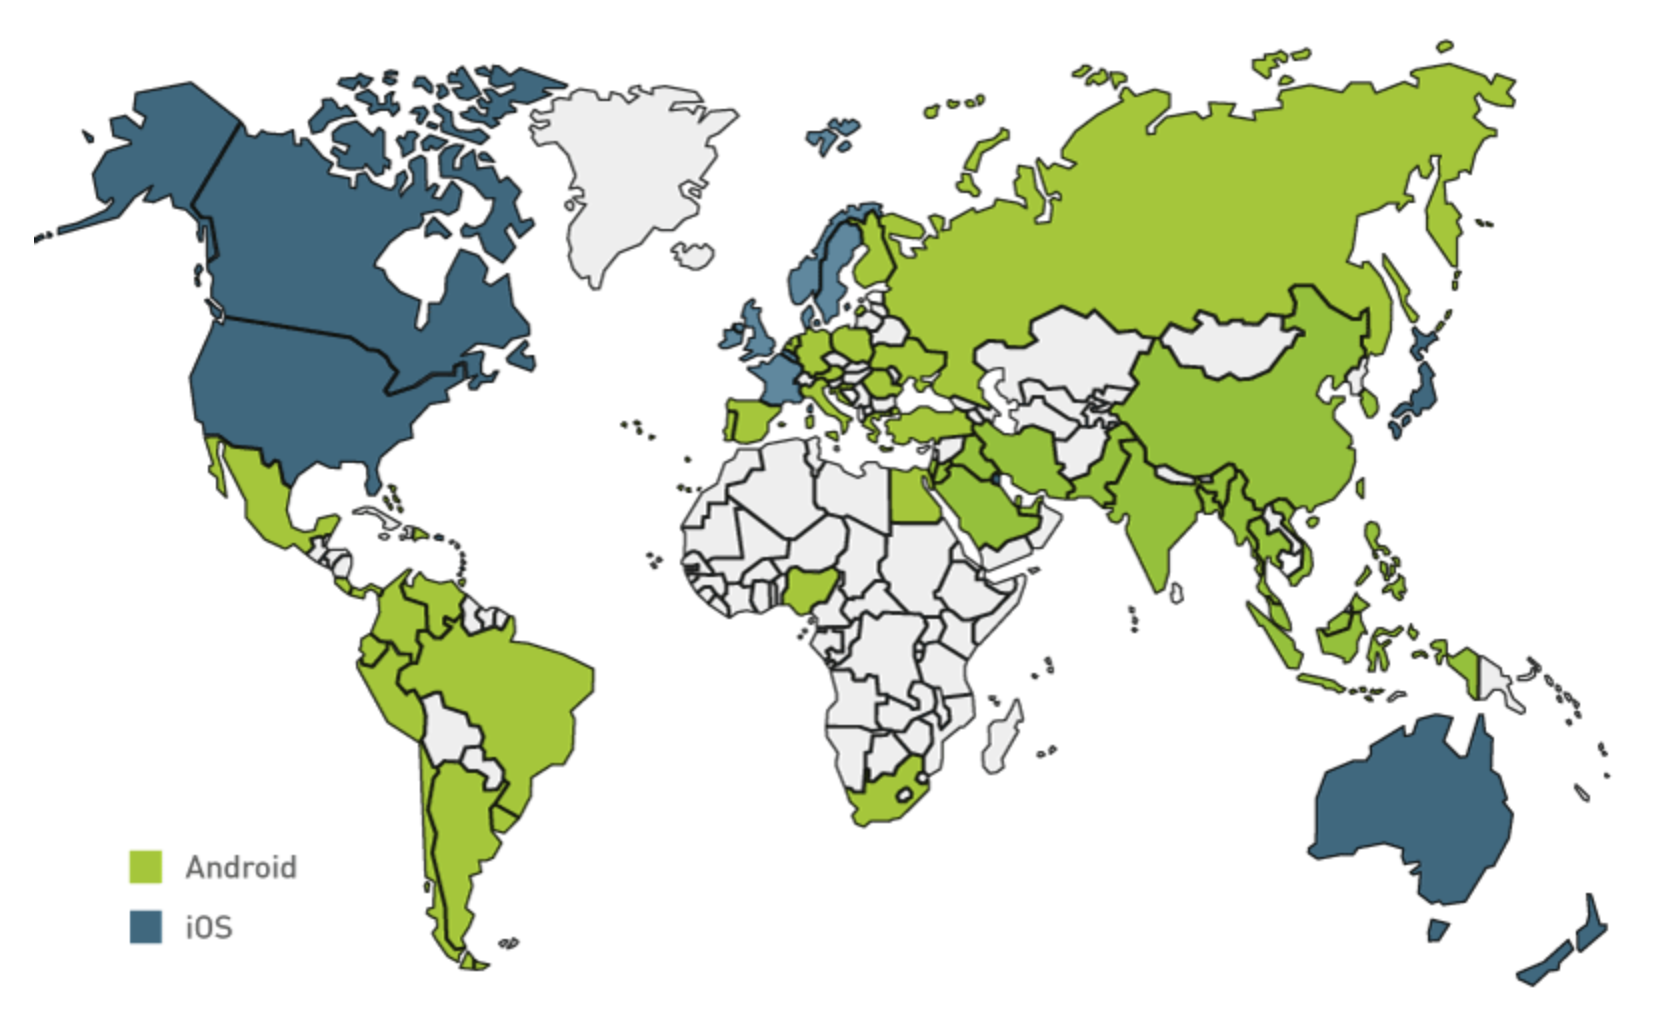
\includegraphics[scale = 0.4] {implementation/marketshare.png}
\end{center}
\caption{Market share (source: App Annie)}
\label{MAP}
\end{figure}
%%%%%%%%%%%%%%%%%%%%%%%%%%%%%%%%%%%%%%%%

Currently there are more active android devices than there are ios devices globally. Knowing real world tests would be required from willing participants, the likelihood of them owning an android device would be marginally higher.
\begin{itemize}
\item Access to hardware
\end{itemize}

The most important factor, Android allows for much better access to the hardware of the device it is installed on, crucial for an application relying on accurate and reliable sensor measurements. Being a less restrictive unix based operating system features such as file management are also possible. The offloading of sensor readings is a simple process through any pc or another android device.


\subsection{Android Studio - Java}

%%%%%%%%%%%%%%%%%%%%%%%%%%%%%%%%%%%%%%%%
\begin{wrapfigure}{l}{0.4\textwidth}
\begin{center}

\includegraphics[scale = 0.3] {implementation/studio-logo.png}
\end{center}

\label{studio}
\end{wrapfigure}
%%%%%%%%%%%%%%%%%%%%%%%%%%%%%%%%%%%%%%%%

Android Studio, being the official IDE for developing android applications and being provided by Google, it was the clear choice. As well as including Github integration for easy version control, Android studio includes useful debugging features such as logcat to view exactly what line of code in which file caused an error. The built in AVD manager allows for testing of code in an emulated android environment, this proved useful for ui changes but does not include sensors or gps leading me to do most of my testing on my own device. Android Studio’s profiler proved useful to help me stay on track in terms of power consumption. Resources such as memory and cpu usage can be monitored on a per activity basis, which ultimately led to some code restructuring to improve device responsiveness in some situations. Android runs java natively, allowing some aspects such as the Logistic Regression class to be developed, tested and optimized on a desktop computer, which with little effort can be copied into the application where it will perform as expected. Investigating the ideal learning rate and number of iterations were also conducted on a computer, which saved a lot of time compiling the application and installing it every time a change was made.   



\subsection{SQLite}

%%%%%%%%%%%%%%%%%%%%%%%%%%%%%%%%%%%%%%%%
\begin{wrapfigure}{r}{0.4\textwidth}
\begin{center}

\includegraphics[scale = 0.5] {implementation/SQLite.png}
\end{center}

\label{sql}
\end{wrapfigure}
%%%%%%%%%%%%%%%%%%%%%%%%%%%%%%%%%%%%%%%%





Databases are crucial to the functionally of RideSafe, using SQLite databases in android allow for secure reliable data Storage. Separate tables contain data such as training data and profile information, crucial datasets for the apps operation.  The usage of cursors allow for easy navigation and data retrieval. The use of a databaseHelper class allowed for the use of simple java functions to perform complex SQL commands, which removed the need to write raw SQL commands more than once.

\subsection{Github}
%%%%%%%%%%%%%%%%%%%%%%%%%%%%%%%%%%%%%%%%
\begin{wrapfigure}{l}{0.5\textwidth}
\begin{center}

\includegraphics[scale = 0.4] {implementation/github.png}
\end{center}

\label{git}
\end{wrapfigure}
%%%%%%%%%%%%%%%%%%%%%%%%%%%%%%%%%%%%%%%%




Github was used for version control for both RideSafe and the data collection app. Github served as a secure backup of work and allowed the author to switch between desktops and laptops in seconds, continuing from exactly where they left off. Branching allowed for major changes with the option to revert back to a working state easily if necessary. Both RideSafe and the data collection version both share a large portion of code, copying the repo and uploading it under a different name when development required allowed for both apps to be developed essentially in parallel and when the time came both apps could be developed separately.   


\subsection{Python}
%%%%%%%%%%%%%%%%%%%%%%%%%%%%%%%%%%%%%%%%
\begin{wrapfigure}{r}{0.5\textwidth}
\begin{center}

\includegraphics[scale = 0.5] {implementation/python-logo.png}
\end{center}

\label{python}
\end{wrapfigure}
%%%%%%%%%%%%%%%%%%%%%%%%%%%%%%%%%%%%%%%%

The source code for RideSafe does not contain a single line of python, however the functions provided in google sheets were limiting what operations that could be done to sort the raw sensor data that was collected. Using python thousands of lines of raw sensor data could be processed and categorized in an instant, ultimately allowing the charastics of crashes to be learnt by analysing sorted data. File combinations also were handled in python, depending on use RideSafe Data Collection App would export multiple files of different runs or one single file with hours of non related data also included. The use of python allowed for hours of manual sorting to be done automatically in seconds.


\section{Main Activities}

This section will discuss in detail the main activities and classes used in the main operation of RideSafe
\subsection{Splash Screen \& Logistic Regression}

%%%%%%%%%%%%%%%%%%%%%%%%%%%%%%%%%%%%%%%%
\begin{wrapfigure}{r}{0.3\textwidth}
\begin{center}
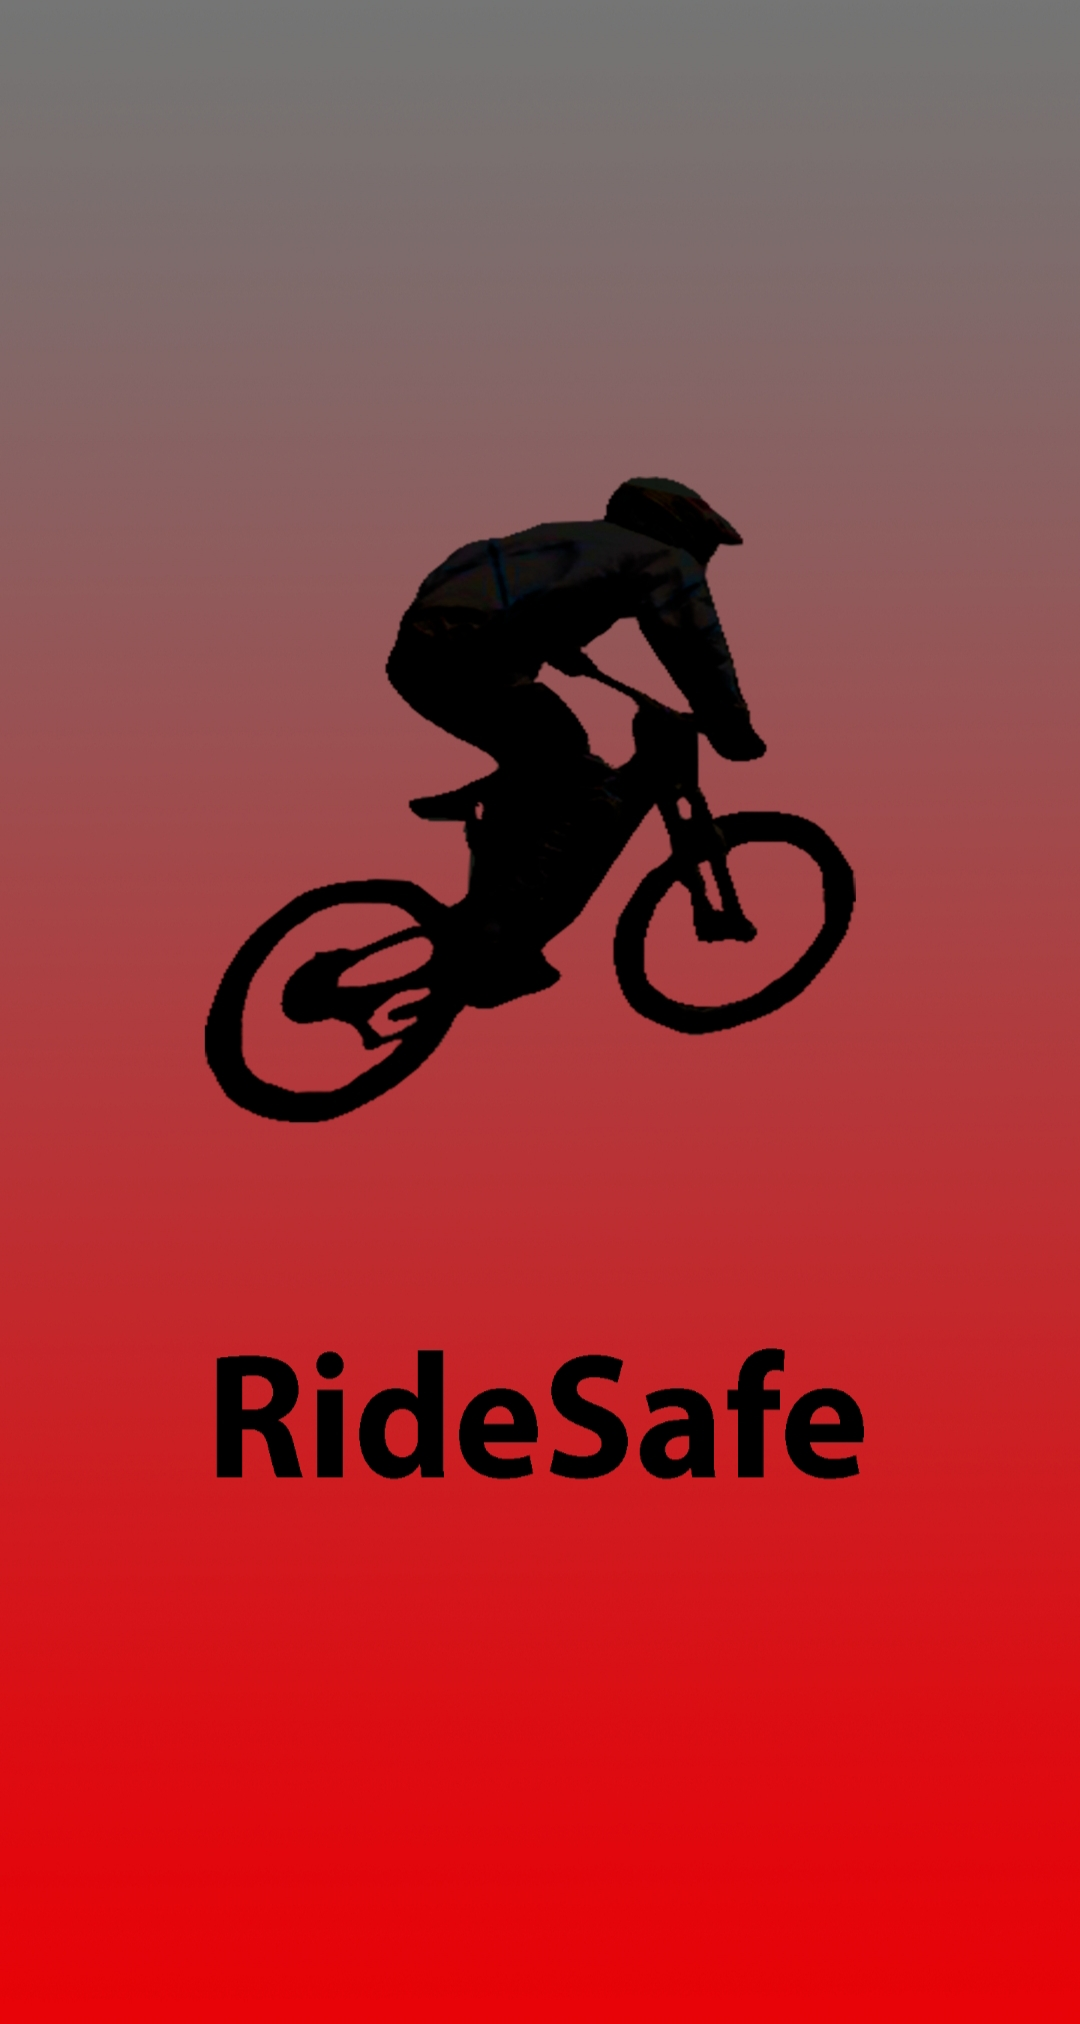
\includegraphics[scale = 0.1] {implementation/splash.jpg}
\end{center}
\caption{A Screenshot of the Slash Screen}
\label{splash}
\end{wrapfigure}
%%%%%%%%%%%%%%%%%%%%%%%%%%%%%%%%%%%%%%%%


To the user the splash screen looks to be simply a loading image as seen in Figure \ref{splash} , but this is not the case. In the background some operations crucial to operation are being carried out. Firstly RideSafe checks if the application has previously been set up by means of a SQLite query, by querying the number of entries of the user profile table, the requirement for setup being required can be determined. If setup is required RideSafe directs the user through the setup process.

\vspace{3cm}


\begin{lstlisting}[language=Java,basicstyle=\small, breaklines=true, label={lst:Code Snippet1},caption={Querying database entries}]
SQLiteDatabase db = mDatabaseHelper.getWritableDatabase();
int tableRows = (int) DatabaseUtils
.queryNumEntries(db, "profile_info");
if (tableRows < 1)
\end{lstlisting}






For performance and stability reasons two major tasks are also run: 



\begin{itemize}
\item{Loading and updating training data.}
\end{itemize}

In the case of either the app is run for the first time or an updated version of the training data is pushed, the training data will be reloaded. The training data supplied with ridesafe is stored as an asset as a text file, the text file, shown in figure \ref{std}, contains the known sensor values of both crashes and normal riding. The final column is the label for the data, used to indicate whether the data corresponds to a crash (1) or a non crash (0). Loading data from a file is expensive in terms of time, so this process is only performed when absolutely necessary. The training data is read in line by line and stored in a SQLite database table. The data provides secure storage and quick access to the data when needed.


%%%%%%%%%%%%%%%%%%%%%%%%%%%%%%%%%%%%%%%%
\begin{figure}[h]
      \centering
      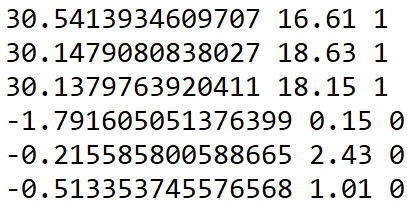
\includegraphics[scale = 1]{implementation/std.png}
      \caption{An Example Of RideSafe Training Data}
      \label{std}
\end{figure}
%%%%%%%%%%%%%%%%%%%%%%%%%%%%%%%%%%%%%%%%

\vspace{1cm}

\begin{lstlisting}[language=Java,basicstyle=\small, breaklines=true, label={lst:labell},caption={Loading Training Data from a file and storing in a database table}]
try (BufferedReader reader = new BufferedReader(
	new InputStreamReader(getAssets().open("TrainingData.txt")))) {
	
	// loop untill eof
	String mLine;
	while ((mLine = reader.readLine()) != null) {
		String[] columns = mLine.split("\\s+");
		double[] data = new double[columns.length];
		for (int i = 0; i < columns.length; i++) {
		data[i] = Double.parseDouble(columns[i]);
                }
           
		ContentValues values = new ContentValues();
		values.put("gforce", data[0]);
		values.put("rotation", data[1]);
		values.put("label",data[2]);
		mDatabaseHelper.addRow(values, "TrainingData");
\end{lstlisting}




\begin{itemize}
\item  {Training the logistic regression model.}
\end{itemize}


Once the data has been loaded for the first time or updated the logistic model needs to be re trained. Testing had shown a very small learning rate of 0.0005 combined with 500 iterations calculated accurate weights for each variable in a training data set containing circa 300 entries. Training data used for Ridesafe will be discussed in section 4.3. A combination of a small learning rate paired with a large number of weight estimate iterations ensures accurate weights can be calculated. In this implementation the weights are along a u-shaped curve, using the learning rate as essentially a step size increases the accuracy of weight estimation. The learning rate can be observed as linearly dependant in respect to the iteration count. If a very large learning rate was used the algorithm could overstep or undershoot  the most accurate weight estimation. The implications of using too few iterations would result in the system terminating prematurely, resulting in incomplete weight estimations.




\begin{lstlisting}[language=Java,basicstyle=\small, breaklines=true, label={lst:train},caption={Training/updating the Model}]
  public void train(DatabaseHelper mDatabaseHelper, int col) {
        Cursor dataCursor = mDatabaseHelper.getData("td");
        int numRows = 0;
        while (dataCursor.moveToNext()){
            numRows++;
        }
        for (int n=0; n<numIterations; n++) {
            dataCursor.moveToFirst();
            for (int i=0; i<numRows; i++) {
                double[] x;
                x = new double[1];
                x[0] = dataCursor.getDouble(col);
                double predicted = classify(x);
                double DataLabel = dataCursor.getInt(3);
                weights[0] = weights[0] + LearningRate * (DataLabel - predicted) * x[0];
                dataCursor.moveToNext();
            }
        }
        System.out.println( Arrays.toString(weights) );
        dataCursor.close();
    }
\end{lstlisting}




Figure \ref{std} shows an example of RideSafes training data, the first column is g-force, followed by change in rotational velocity and finally the assigned label.
For each row in the training data training table of the database,  the value is classified based on the current calculated weight (var predicted). Then the weight for that sensor reading is recalculated based on what the system has already learnt, with the exception of iteration 0 where the predicted value will be 50\% likely. 
  weights[i] = weights[i] + Learning Rate * (DataLabel - predicted) * x[i];
The current weight for sensor data i = the current weight for sensor data i + the specified learning rate(0.0005) * (The known class of the variable either 1 for a crash or 0 otherwise - what it currently classifies as) * the sensor reading associated with that weight. This process is repeated until the weights are as accurate as possible and no longer change. The final calculated Weights for both g-force \& total rotational velocity change from the training data used can be seen in figure \ref{weights}. The regression model provides an answer to the following in real-time, Given current sensor values x , what is the probability of (1|x) where 1 is the class label belonging to data pre-learnt of accidents.




%%%%%%%%%%%%%%%%%%%%%%%%%%%%%%%%%%%%%%%%
\begin{figure}[h]
      \centering
      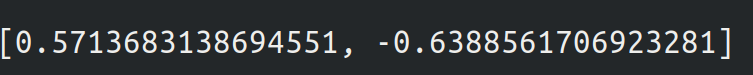
\includegraphics[scale = .5]{implementation/weights.png}
      \caption{Weights calculated by the Multivariate Logistic Model}
      \label{weights}
\end{figure}
%%%%%%%%%%%%%%%%%%%%%%%%%%%%%%%%%%%%%%%%

\vspace{2cm}

The function used for classification as shown below is an implementation of the formula for the sigmoidal Logistic curve  \[
    P = \frac{1}{1+e^ -(a+bX)}
\]   For Each Row of data the probability P is calculated using the logistic curve.


\begin{lstlisting}[language=Java,basicstyle=\small, breaklines=true, label={lst:labell},caption={Classify Function}]

 public double classify(double[] x) {
        double logit = .0;
        for (int i=0; i<weights.length;i++)  {
            logit += weights[i] * x[i];
        }
        return 1.0 / (1.0 + Math.exp(-logit));
    }
\end{lstlisting}





As seen in figure \ref{logit} green points on the graph are plotted with a probability near 0, these points represent the sensor values associated with a non crash. The red points are plotted probabilities of sensor values representing crashes. The blue point represents classified sensor values with no known truth, using the learnt weights the model calculates the probability of the likelihood the readings match those of an accident, e, g,. The sensor values related to the blue dot are more similar to what the system knows is a crash, resulting in a high probability that a crash has occurred. 






%%%%%%%%%%%%%%%%%%%%%%%%%%%%%%%%%%%%%%%%
\begin{figure}[h]
      \centering
      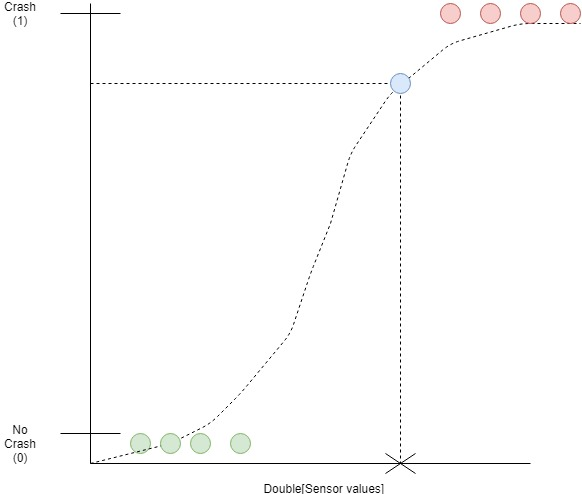
\includegraphics[scale = .6]{implementation/logit.jpg}
      \caption{Sigmoid curve produced by a logit function}
      \label{logit}
\end{figure}
%%%%%%%%%%%%%%%%%%%%%%%%%%%%%%%%%%%%%%%%


\vspace{3cm}




%%%%%%%%%%%%%%%%%%%%%%%%%%%%%%%%%%%%%%%%
\begin{figure}[h]
      \centering
      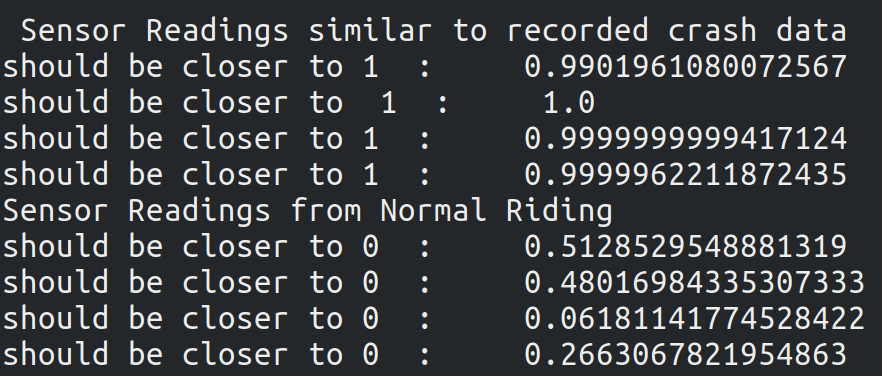
\includegraphics[scale = .5]{implementation/tv.png}
      \caption{Classifying Example Test values With A Trained Model}
      \label{tv}
\end{figure}
%%%%%%%%%%%%%%%%%%%%%%%%%%%%%%%%%%%%%%%%



Figure \ref{tv} shows example test cases of both crash and non crash data being classified, Crash data is quite unique versus standard riding data leading to crashes being identified to a high degree of certainty, Normal Riding varies quite a lot leading to a range of output probabilities. 



\newpage
\subsection{Home Screen}


%%%%%%%%%%%%%%%%%%%%%%%%%%%%%%%%%%%%%%%%
\begin{wrapfigure}{r}{0.3\textwidth}
\begin{center}
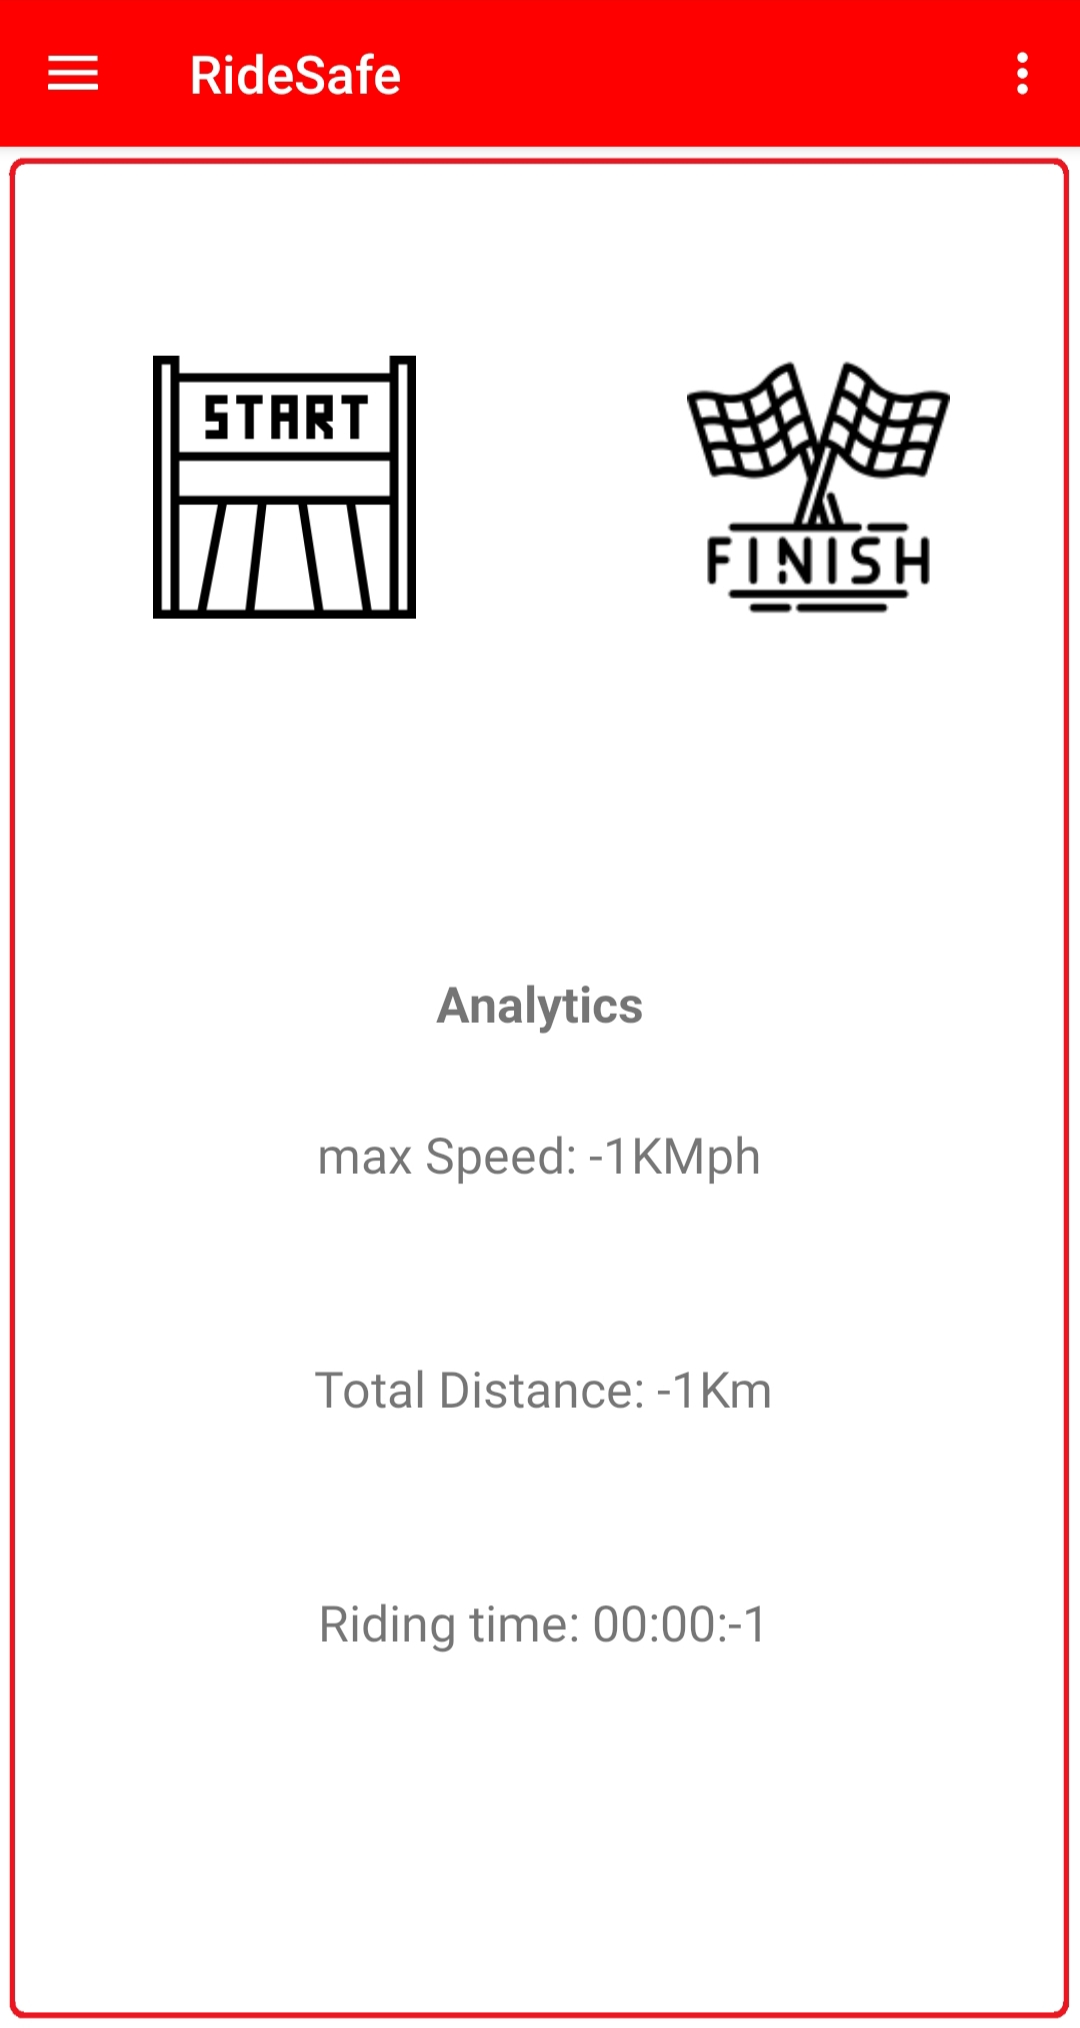
\includegraphics[scale = 0.15] {implementation/home.jpg}
\end{center}
\caption{A Screenshot of the home Screen}
\label{homescreen}
\end{wrapfigure}
%%%%%%%%%%%%%%%%%%%%%%%%%%%%%%%%%%%%%%%%


The author kept the home screen as simple and user friendly as possible. By utilizing large black icons against a plain white background the screen remains viewable in extremely bright and dark environments. Buttons were kept large for ease of use while wearing gloves as many cyclists do. Towards the bottom of the screen are some useful analytics for the user such as their max recorded speed \& distance traveled. 


\begin{lstlisting}[language=Java,basicstyle=\small, breaklines=true, label={lst:labellll},caption={Starting the Crash Detection Service}]

public void startService(View v) {

        locationManager = (LocationManager) getSystemService(LOCATION_SERVICE);
        gpsManager = new GPSConfig(main_Home.this);
        isGPSon = locationManager.isProviderEnabled(LocationManager.GPS_PROVIDER);

        if (isGPSon) {
            String init = "running";
            Intent serviceIntent = new Intent(this, RideSafeService.class);
            serviceIntent.putExtra("inputExtra", init);
            startService(serviceIntent);
            RUNNING = true;
        } else {
            showSettingsAlert();
        }
    }
\end{lstlisting}

On Pressing the Start Button RideSafe performs a check to determine if location services are enabled for the device. If GPS is not enabled the user is prompted to do so in their device settings, otherwise an intent is launched to start the background service which will be discussed in detail in the next section. 
The Stop service button is simply the opposite of the start button bar the gps check, An intent is launched on pressing the to end the background service. The analytics section is also updated on pressing finish.  










\subsection{RideSafe Background Service}

%%%%%%%%%%%%%%%%%%%%%%%%%%%%%%%%%%%%%%%%
\begin{wrapfigure}{r}{0.2\textwidth}
\begin{center}
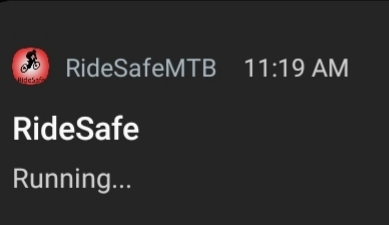
\includegraphics[scale = 0.2] {implementation/service.jpg}
\end{center}
\caption{A Screenshot of the service notification}
\label{crash}
\end{wrapfigure}
%%%%%%%%%%%%%%%%%%%%%%%%%%%%%%%%%%%%%%%%

RideSafes background service is where both all the sensor monitoring takes place and the rule based system is implemented. On pressing the start button on the home screen the background service is launched. This background service has no view or user interface layout, the user is reassured the system is running  with a persistent device notification which can be seen in figure (ref), Google recently required any background service to have a notification displayed to inform the user operations are being performed which cannot be seen.



 \begin{lstlisting}[language=Java,basicstyle=\small, breaklines=true, label={lst:labell},caption={Taking Sensor Readings}]

@Override
    public void onSensorChanged(SensorEvent event) {

        sensorType = event.sensor.getType();
        if (sensorType == 1 && !GAquired) {     // accelerometer
            X = event.values[0];
            Y = event.values[1];
            Z = event.values[2];
            ACCELEROMETER = Math.sqrt(X * X + Y * Y + Z * Z) - 9.807;
            ACCELEROMETER = (double)Math.round(ACCELEROMETER * 100d)/100d;
            GAquired = true;

            if(RAquired) {
                GAquired = false;
                RAquired = false;
                ClassifyX();
            }
        } else if (sensorType != 1 && !RAquired) {

            GYROX = event.values[0];
            GYROY = event.values[1];
            GYROZ = event.values[2];

            GYROX = (double)Math.round(event.values[0] * 100d)/100d;
            GYROY = (double)Math.round(event.values[1] * 100d)/100d;
            GYROZ = (double)Math.round(event.values[2] * 100d)/100d;
            currentRot = GYROX + GYROY + GYROZ / 3;
            currentRot = (double)Math.round(currentRot * 100d)/100d;

            RAquired = true;
            if(GAquired){
                GAquired = false;
                RAquired = false;
                ClassifyX();
            }

        }
    }

\end{lstlisting}



 \begin{lstlisting}[language=Java,basicstyle=\small, breaklines=true, label={lst:labell},caption={Senor Setup}]


SM.registerListener(this, myAccelerometer, SensorManager.SENSOR_DELAY_NORMAL);
        SM.registerListener(this, myGyroscope, SensorManager.SENSOR_DELAY_NORMAL);

\end{lstlisting}



The recording of sensor values is performed as shown above in lstlisting Sensor Readings In the onCreate method both the accelerometer and gyroscope are initialized as well as registering device listeners. As both sensors are required to use the same onsensorchanged method booleans are used as triggers similar to the operation of a basic state machine. When readings from both sensors have been acquired they are converted into the required format as discussed previously in the design section. The next reading required is the current speed.


 \begin{lstlisting}[language=Java,basicstyle=\small, breaklines=true, label={lst:labell},caption={Calculating Speed \& Distance}]


@Override
    public void onGPSUpdate(Location location) {
        speed = location.getSpeed();
        currentSpeed = round(speed, 3, BigDecimal.ROUND_HALF_UP);
        SPEEDCURR = round((currentSpeed * 3.6), 3, BigDecimal.ROUND_HALF_UP);
        if((int)SPEEDCURR > MaxSpeed){
            MaxSpeed =  (int)SPEEDCURR;
        }
        if(prev.getLatitude() != -9999 && prev.getLongitude() != -9999){
            current.setLatitude(location.getLatitude());
            current.setLongitude(location.getLongitude());
            distance = (int) current.distanceTo(prev);
            distance = distance / 1000;
            TotalDistance = TotalDistance + distance;
            ContentValues values = new ContentValues();
            values.put("lat", current.getLatitude());
            values.put("long", current.getLongitude());
            values.put("speed", SPEEDCURR);
            mDatabaseHelper.addRow(values, "locationData");
            prev.setLatitude(current.getLatitude());
            prev.setLongitude(current.getLongitude());
        }
        else{
            prev.setLatitude(location.getLatitude());
            prev.setLongitude(location.getLongitude());
        }
    }

\end{lstlisting}


Speed is calculated using android's location services, utilizing location services speed is calculated by means of distance over time, where distance is the straight line distance between two locations, each location is in the form of a latitude-longitude pair and factoring in the curvature of the earth a suitably accurate speed and distance can be calculated. As RideSafe is intended to be used in areas which may not have the best signal, the location manager will fall back to cell tower triangulation to compute a location if no GPS signal is available. SPEEDCURR is speed converted to kilometer per hour and rounded to three decimal places as a huge degree of accuracy is not required. Latitudes and longitudes as well as the speed to which was being travelled is also computed and recorded for the purpose of journey tracking which is an option available in the maps section of the application. Both the polling for the  accelerometer and gyroscope is far quicker than calculating speed, speed is on average three times slower to calculate than g-force and rotational velocity are, leading to 3 calculations of each sensor corresponding to a single speed.       


 \begin{lstlisting}[language=Java,basicstyle=\small, breaklines=true, label={lst:labell},caption={RideSafe’s Rule Based System}]

 public void ClassifyX() {

        if (ACCELEROMETER != nullNum && GYROX != nullNum && GYROY != nullNum && GYROZ != nullNum && SPEEDCURR != nullNum) {

            RotChange = currentRot + totalRotPrev;
            RotChange = (double)Math.round(RotChange * 100d)/100d;
            double[] currentGFORCEValue = {ACCELEROMETER};
            double[] currentROTValue = {RotChange};

if(currentGFORCEValue != null && currentROTValue != null) {

    if (!isMoving()) {

        if (LOGISTICG.classify(currentGFORCEValue) < Threshold  && LOGISTICR.classify(currentROTValue) < Threshold)
            Log.d("Answer from service", "No Crash Detected");

        else {
            Log.d("Answer from service", "Crash Detected " );
            monitorSpeed();


        }
    }
}
 
\end{lstlisting}

Once all three parameters are obtained RideSafes system rule is queried to see if an accident may have occurred. The code above implements the following rule:  IF the rider is moving THEN Classify current sensor readings, IF the probability computed based on current readings is less than A threshold THEN a crash has not occured.  IF the probability exceeds the the threshold THEN monitor speed.  All sensor values are classified in real time with a pre trained model. The current speed is not classified in the logistic model as a given speed is valid for both crashes and non crashes, from my testing including speed as a variable in the model produces a calculated weight close to 0.5 as it can be associated with both classes ,leading to its removal. If the threshold is exceeded MoniorSpeed() is called. In this case the rider has experienced a large impact and or excessive rotation. monitorSpeed() Starts a timer rechecking the speed of the rider. If the riders speed has dropped significantly after a large impact from my research one can come to the conclusion an accident has occurred.  If the timer elapses the crash handler which will be discussed in the next section will be launched.

When the service is stopped from the home screen parameters such as riding time and max speed are updated using shared preferences.  Sensors are unregistered and the background service is destroyed. 




\subsection{Crash Handler}



%%%%%%%%%%%%%%%%%%%%%%%%%%%%%%%%%%%%%%%%
\begin{wrapfigure}{r}{0.3\textwidth}
\begin{center}
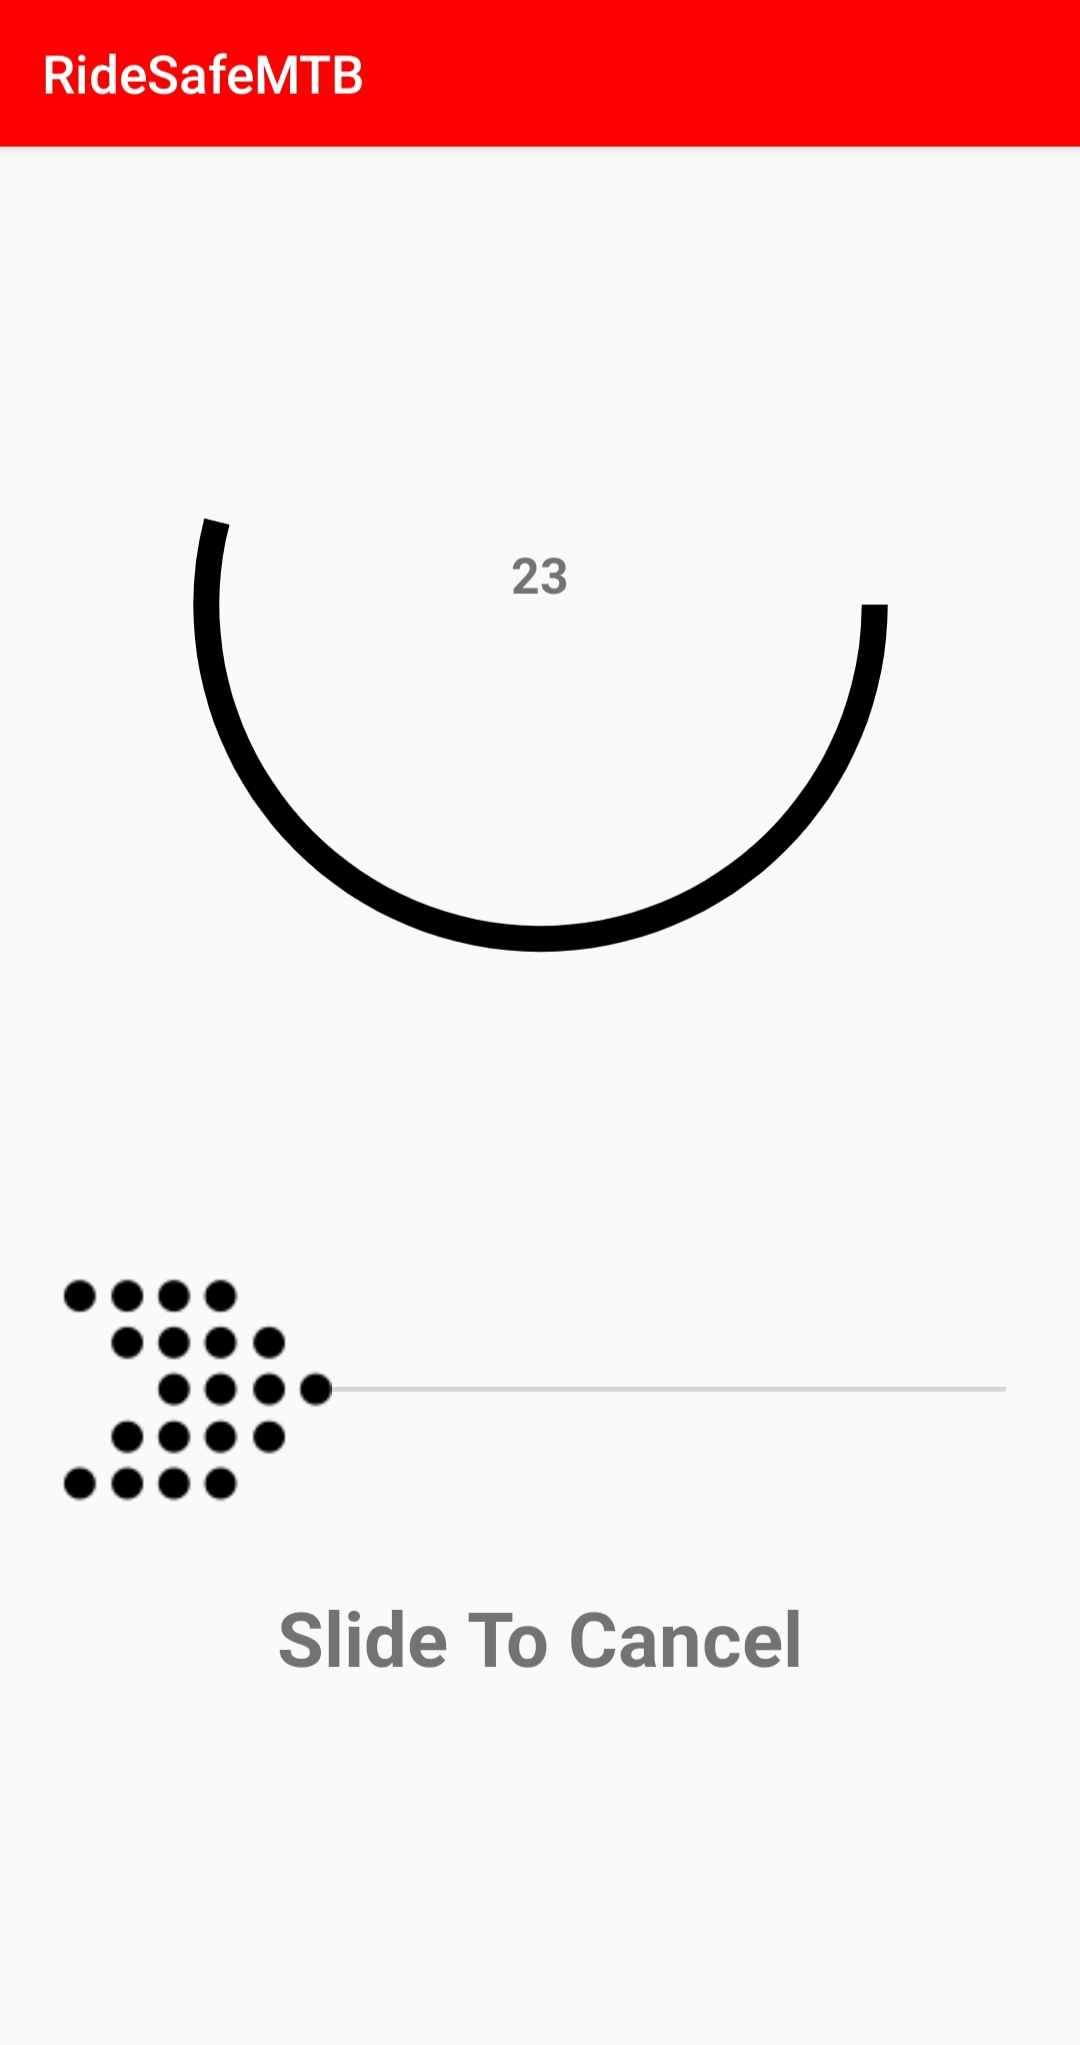
\includegraphics[scale = 0.15] {implementation/crash.jpg}
\end{center}
\caption{A Screenshot of the Crash Handler}
\label{crash}
\end{wrapfigure}
%%%%%%%%%%%%%%%%%%%%%%%%%%%%%%%%%%%%%%%%



figure \ref{crash} shows the layout of the crash handling screen, The crash handler is launched by means of an intent from the background service previously discussed as shown below. The location and speed of where the crash occurred is passed via a bundle for usage in both the accident heatmap and for content in the automatic SMS which is sent.

 \begin{lstlisting}[language=Java,basicstyle=\small, breaklines=true, label={lst:labell},caption={Launching the Crash Handler}]



void LaunchCrashHandler(){
        Intent intent = new Intent(RideSafeService.this, Crash_Handler.class).setFlags(Intent.FLAG_ACTIVITY_NEW_TASK);
        Bundle b = new Bundle();
        b.putDouble("latitude", current.getLatitude());
        b.putDouble("longitude", current.getLongitude());
        b.putDouble("speed", SPEEDCURR);
        intent.putExtras(b);
        startActivity(intent);

    }


\end{lstlisting}

As the crash handler is launched while the users phone is  out of hand and the device locked, extra flags were set for the activity so that it can be launched and displayed from a locked device. By passing the users lockscreen the crash handler is displayed an an audible alarm is played on repeat.Password,pin entry or fingerprint scanning is all bypassed when the activity is launched. The alarm is for the scenario where a false positive my occur to alert the rider to cancel the timer before the sms is sent.
The flags used were as follows:
 \begin{lstlisting}[language=Java,basicstyle=\small, breaklines=true, label={lst:labell},caption={Flags to allow device to RideSafe to display the crash handler}]




 this.getWindow().setFlags(WindowManager.LayoutParams.FLAG_FULLSCREEN |
                        WindowManager.LayoutParams.FLAG_DISMISS_KEYGUARD |
                        WindowManager.LayoutParams.FLAG_SHOW_WHEN_LOCKED |
                        WindowManager.LayoutParams.FLAG_TURN_SCREEN_ON,
                WindowManager.LayoutParams.FLAG_FULLSCREEN |
                        WindowManager.LayoutParams.FLAG_DISMISS_KEYGUARD |
                        WindowManager.LayoutParams.FLAG_SHOW_WHEN_LOCKED |
                        WindowManager.LayoutParams.FLAG_TURN_SCREEN_ON);

\end{lstlisting}


While the alarm is played, a countdown timer is displayed on screen along with a slide bar used to cancel the countdown. In the event of a false positive or an accident where the rider does not require assistance, sliding the cancel slider will cancel the timer and relaunch the background service and re locking the device. A slider is used as it is much more unlikely to accidentally slide to cancel compared to just pressing  a button.


Once the timer expires the users chosen emergency contact is automatically sent an SMS e, g,.  I have had an accident. my location is :https://maps.google.com/?q=" + Latitude + "," + Longitude   "I Crashed while traveling at : " + Speed + "kmph   Sent Automatically by RideSafe".   The users speed and location which were passed from the service intent are used to automatically generate a link to their location on google maps, allowing the emergency contact to relay the information to the authorities, or simply by clicking the link receive directions to accident site themselves. 

 \begin{lstlisting}[language=Java,basicstyle=\small, breaklines=true, label={lst:labell},caption={Automatic SMS Sending}]


private void sendSms() {
        SmsManager smsManager = SmsManager.getDefault();
        smsManager.sendTextMessage(PhoneNumber, null, message, null, null);
        Toast.makeText(getApplicationContext(), "SMS sent to " + ContactName,
                Toast.LENGTH_LONG).show();


    }
\end{lstlisting}


\newpage


\subsection{Settings}

%%%%%%%%%%%%%%%%%%%%%%%%%%%%%%%%%%%%%%%%
\begin{wrapfigure}{r}{0.3\textwidth}
\begin{center}
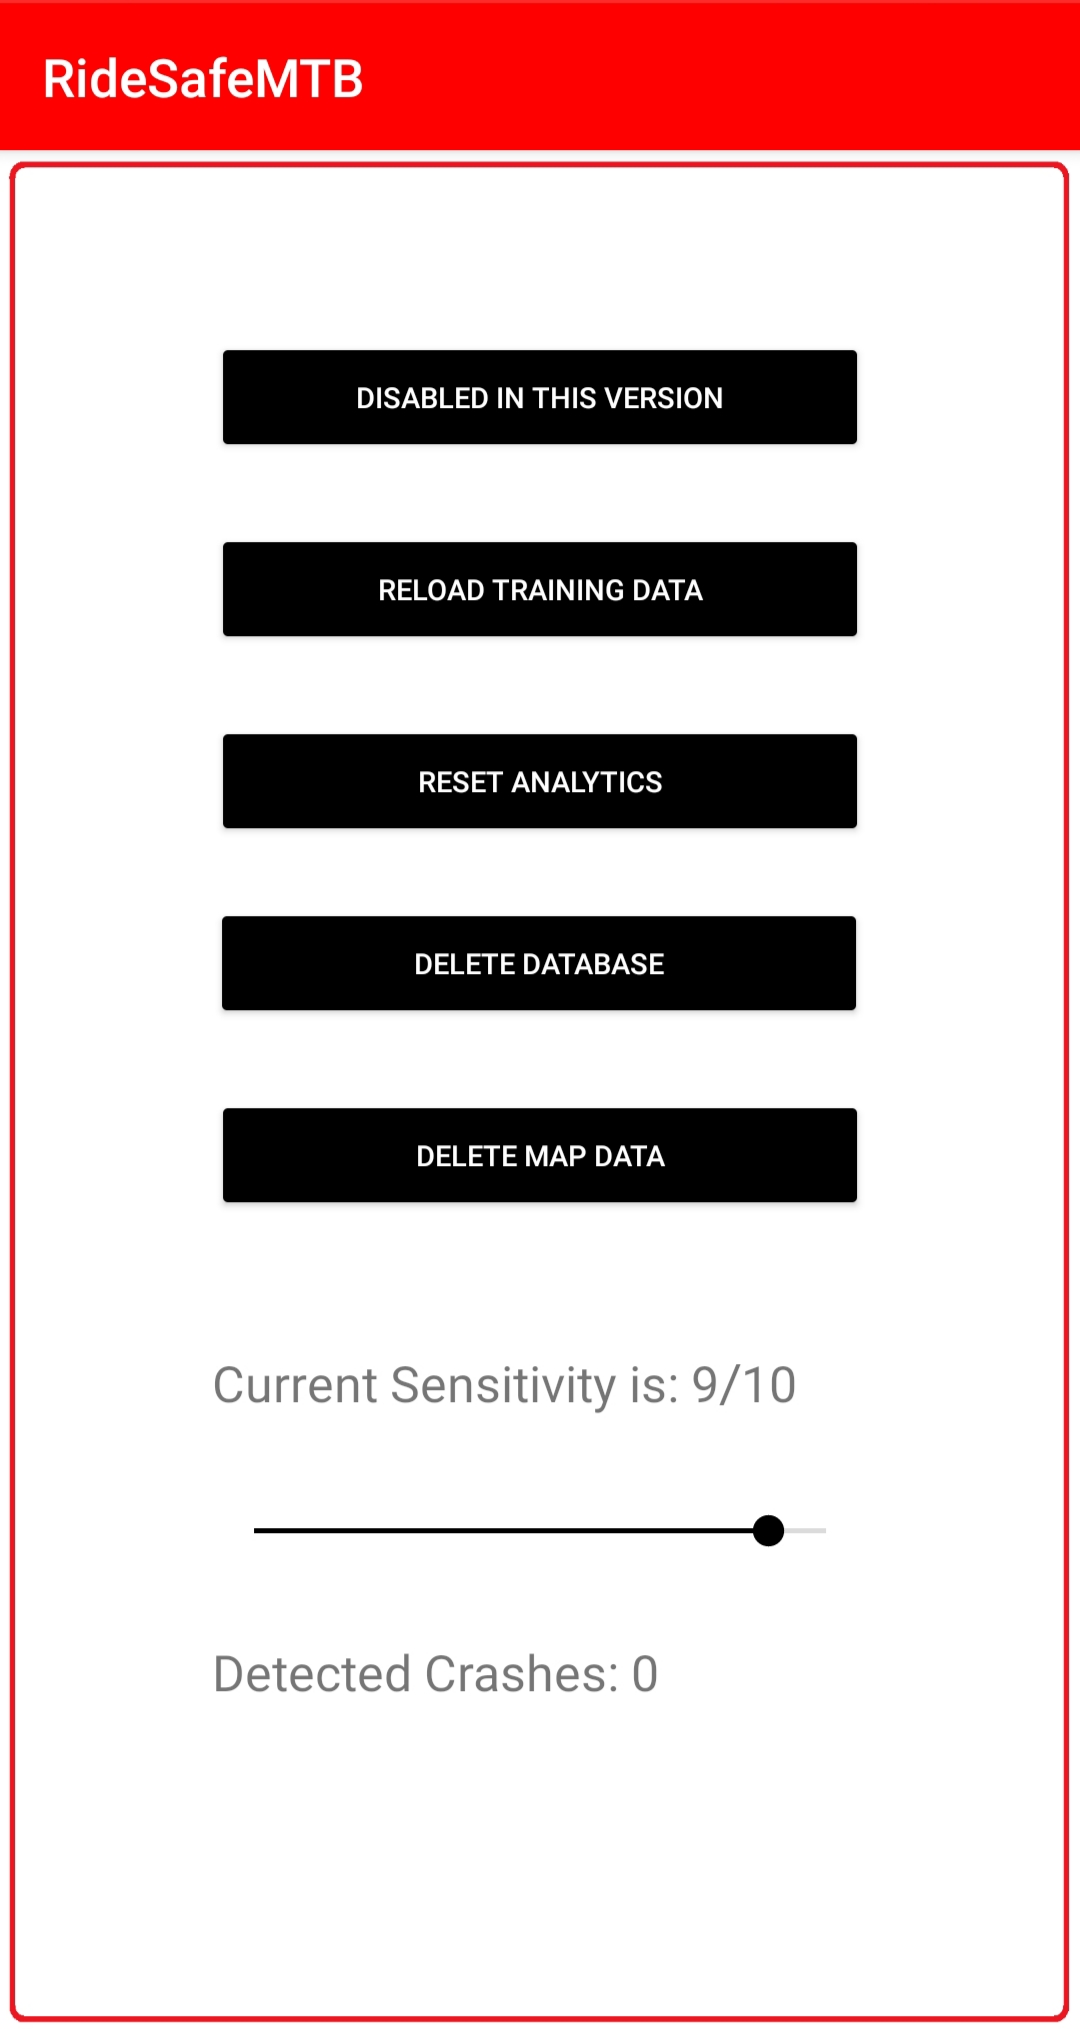
\includegraphics[scale = 0.15] {implementation/set.jpg}
\end{center}
\caption{A Screenshot of the Settings Screen}
\label{set}
\end{wrapfigure}
%%%%%%%%%%%%%%%%%%%%%%%%%%%%%%%%%%%%%%%%

The settings screen as seen in Figure \ref{set}, provides a few useful functions to the end user:

As this screenshot is from the version currently listed on google play the function “export data to the developer” has been disabled in the store version.  The button was originally implemented for allowing quick transfering of sensor data. Upon pressing the button the full database of RideSafe was saved as a database file which was sharable in the android operating system. Data could easily be transferred via email for debugging purposes. Delete Database is closely related and was used in conjunction with the export button to allow small samples of data to be recorded and then deleted, allowing for small separate files rather than a single large file to be exported.

Reload Training data is a manual override to reload and re train the system,  When crashes occur the values associated are added to the systems database, at a convenient time for the user the values are added to the classifier and the system can be retrained.

Reset Analytics and Delete map data are both implemented to clear user specific data such as previous journey latitudes and longitudes used to plot journeys on the map or the max speed displayed on the home screen.

As mentioned in the discussion of the background service, there exists a threshold value for the probability required to trigger a detected crash, the settings screen includes a sensitivity slider to adjust the threshold value used. Each notch on the slider increments or decrements this value by .05, allowing users slight adjustment to improve their experience while using the supplied training data.

The detected crash counter, used for testing purposes is a counter of how many times the application has detected an accident. 


\section{Non-Functional Requirements Implemented}
\vspace{3cm}


%%%%%%%%%%%%%%%%%%%%%%%%%%%%%%%%%%%%%%%%
\begin{figure}[h]
      \centering
      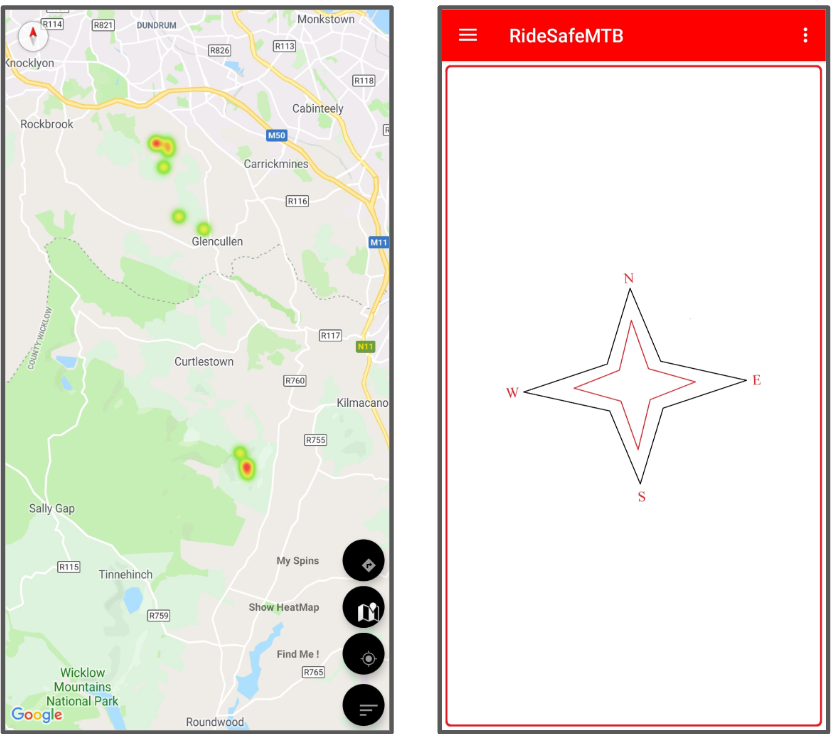
\includegraphics[scale = .9]{implementation/cm.png}
      \caption{Accident HeatMap (left), Compass (Right)}
      \label{cm}
\end{figure}
%%%%%%%%%%%%%%%%%%%%%%%%%%%%%%%%%%%%%%%%

\subsection{Google Maps}

Google's map API was taken utilized to implement two additional features:
\begin{itemize}
\item Accident heatmap 
\end{itemize}

Users can currently see potential danger zones where previous accidents have occured. Once a crash has been detected the users latitude and longitude of where the crash has occurred is plotted on RideSafes built in map. As the size and colour of the spot on the map increases the likelihood of present danger increases. By viewing the map users could decide to take extra caution while passing through the area, or avoid it entirely, potentially preventing an accident occurring. Currently the heatmap is user specific, future plans for the heatmap will be discussed in future work.   

\begin{itemize}
\item Ride Tracking
\end{itemize}
A Simple way to view trails and journeys ridden by the user. By storing the latitudes and longitudes where the rider has travelled in a database table, these points can be plotted on the map allowing the user to view places they have been and passed by. The speed of which the rider was travelling at the certain locations was also recorded with the intention to change the colour of the plotted journey according to the recorded speed however, due to time constraints dynamic line colouring has yet to be implemented.





\subsection{Compass}





With Certain trails being situated in very remote areas, navigation can sometimes be an issue, especially when a connection to the internet cannot be obtained. Using the orientation sensor the direction of magnetic north can be calculated. By simply rotating an image with offsets calculated to point north a very simple yet reliable compass has been implemented. A small but useful feature.








\section{Training}



The Logistic model utilized in RideSafe has been trained by collecting training data in two seperate ways:
\begin{itemize}
\item Logging of ride Data 
\end {itemize}

In the early stages of development data was collected solely by the author while mountain biking at local trail centres. Similar to medical solutions the “ADL” of mountain biking had to be identified and the patterns learnt. Globally trails are allocated a rating to how technical and difficult they are, ranging from a “green” trail to “double black diamond”. Thousands of points of data were collected from “blue” “red” \& “black” trails in the Dublin/Wicklow area. This data proved invaluable in terms of learning what are considered “normal” sensor readings while mountain biking. Upon receiving ethical approval data has been collected from numerous riders of varying skill level and experience.
\begin{itemize}
\item Crashing in a controlled environment
\end{itemize}
For the model not to be biased an equal number of instances of both crash data and non crash data must be present in the training data, With few “real World” major accidents occurring during the data collection phase action was taken to ensure the system could be trained correctly. Alike the training performed in medical applications where controlled falls are purposely done onto a soft surface such as a mattress, the author conducted similar tests at the local indoor skate park.
Three hours of intentional crashes were performed in one of two main ways: The most common cause of severe mountain biking injury - over the handlebars as well as side impact which is commonly caused by loss of traction.    







Figure \ref{fall} shows stills of a video taken with accompanying sensor readings closely aligned. The sample rate used was 3 readings of each sensor per second bar speed which is slower to calculate ( roughly once per second). The data readings are labelled and are displayed over time.
 The first section closely resembles data collected from normal riding on a green trail, slow speed, low g-force and marginal rotation of the device. 
Section 2 closely resembles data collected from riding blue/red trails, spikes in both g-force and rotation of the device, more movement in terms of rotational velocity on all axis as well as spikes in g-force. In this instance the spikes are caused by the small direction change associated riding the takeoff ramp.
Section 3 \& 4 are of most interest, the flatline from the sensor values are caused by gliding through the air, completely off the ground. Section 4 is both impact and aftermath. Big spikes of both g-force and rotational velocity can be observed as impact occurs. As clear from the graph the change in speed is a huge anomaly compared to standard riding. The results of this testing allowed for the development of RideSafe’s rule base.

After countless intentional falls enough data was collected to both identify the characteristics and pattern of the events occuring during an accident.  




%%%%%%%%%%%%%%%%%%%%%%%%%%%%%%%%%%%%%%%%
\begin{figure}[h]
      \centering
      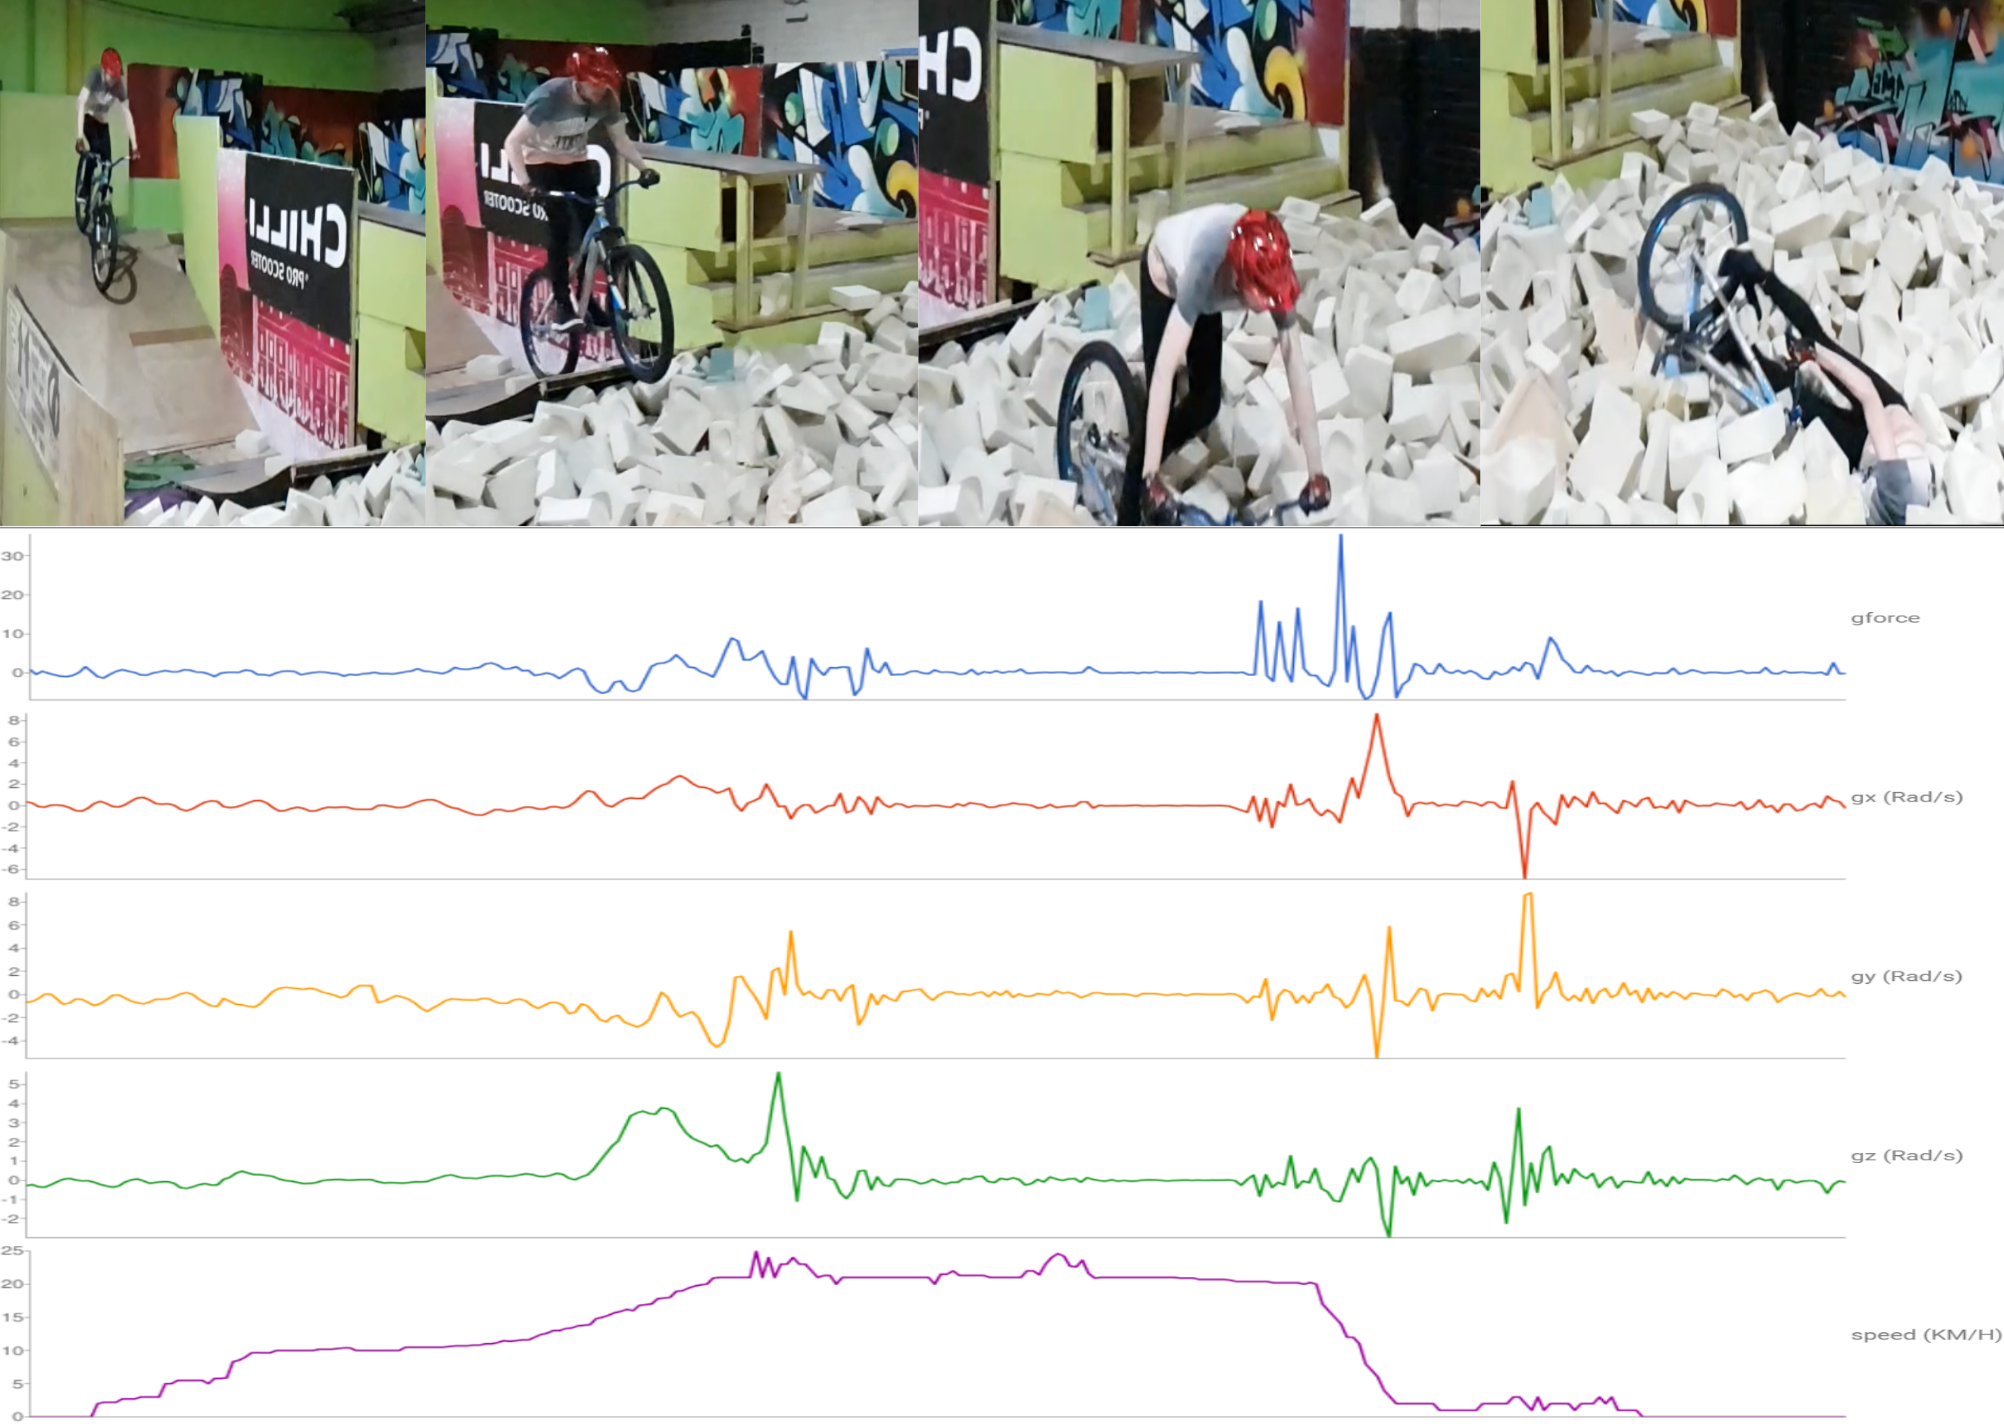
\includegraphics[scale = .6]{implementation/fall.png}
      \caption{Analysis of A Crash}
      \label{fall}
\end{figure}
%%%%%%%%%%%%%%%%%%%%%%%%%%%%%%%%%%%%%%%%SS

\newpage
\section {Application Flow Diagram}


%%%%%%%%%%%%%%%%%%%%%%%%%%%%%%%%%%%%%%%%
\begin{figure}[h]
      \centering
      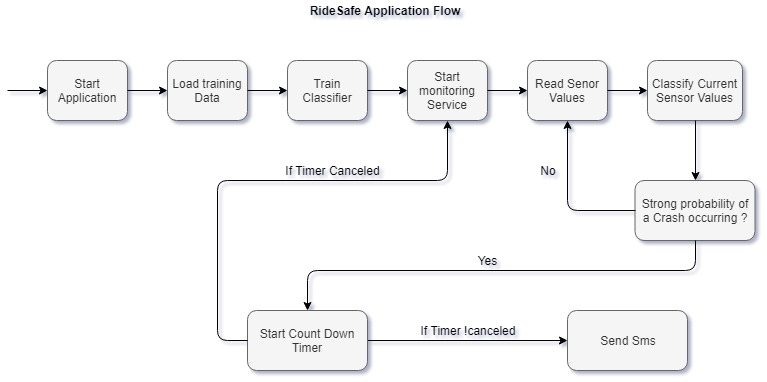
\includegraphics[scale = .6]{implementation/flow.jpg}
      \caption{RideSafe Application Flow}
      \label{flow1111}
\end{figure}
%%%%%%%%%%%%%%%%%%%%%%%%%%%%%%%%%%%%%%%%SS







%%\chapter{\LaTeX}
\label{latexchapter}
seeing \LaTeX{}, or more properly ``\LaTeXe{}'', is a very useful document processing program. It is very widely used, widely available, stable and free. Famously, \TeX, upon which \LaTeX{} is built, was originally developed by the eminent American mathematician Donald Knuth because he was tired of ugly mathematics books\cite{shustek2008interview}. Although it has a learning curve (made much less forbidding by online tools and resources -- see below), it allows the writer to concentrate more fully on the content, and takes care of most everything else.

While it can be used as a word processor, it is a \emph{typesetting} system, and Knuth's idea was that it could be used to produce beautiful looking books:
\begin{quote}
\emph{\LaTeX{} is a macro package which enables authors to typeset and print their work at the highest typographical quality, using a predefined, professional layout.}\footnote{This is from \citet{oetiker2001not}. Did we mention that you should minimise your use of footnotes?}
\end{quote}
\LaTeX{} has great facilities for setting out equations and a powerful and very widely supported bibliographic system called BibTeX, which takes the pain out of referencing.

Three useful online resources make \LaTeX~much better:
\begin{enumerate}[(1)]
\item An excellent online \LaTeX{} environment called ``Overleaf'' is available at \url{http://www.overleaf.com} that runs in a modern web browser. It's got this template available -- search for a TCD template. Overleaf can work in conjunction with Dropbox, Google Drive and, in beta, GitHub.
\item Google Scholar, at \url{http://scholar.google.com}, provides BibTeX entries for most of the academic references it finds.
\item An indispensable and very fine introduction to using \LaTeX{} called \emph{``The not so short introduction to LATEX 2$\varepsilon$''} by \citet{oetiker2001not} is online at \url{https://doi.org/10.3929/ethz-a-004398225}. Browse it before you use \LaTeX~for the first time and  read it carefully when you get down to business.
\end{enumerate}
Other tools worth mentioning include:
\begin{itemize}
\item \texttt{Draw.io} -- an online drawing package that can output PDFs to Google Drive -- see \url{https://www.draw.io}.
\end{itemize}
\chapter{Evaluation}

\chapter{Conclusion}

\section {Future Work}

\subsection {Training}

The author believes that the accuracy of RideSafes detection algorithm could greatly be improved with more comprehensive training data. Due to time constraints the data used for training the machine learning model is not as diverse as intended. The training data used for ride safe during tested was collected only from two riders. As discussed throughout even with the most common types of crashes displaying similar patterns, no two riders are identical.   With RideSafe performing as it does one can only deduce performance would improve with a more generalized model to begin with eventually leading to a more personalized model over time.





\subsection {Collaboration}

Currently on the market popular ride tracking applications severely lack  any safeguards for the users safety, popular cycling oriented fitness tracking applications such as Trailforks or Strava actively monitor the users speed and location. Without major redesigns for either party the crash detection logic present in RideSafe could be implemented as a supplementary feature for the benefit of the users. Since the most power intensive feature of RideSafe is GPS functionality, the algorithm could be added to Strava or Trailforks adding only marginally higher power consumption then they already have.




\subsection {Inter-Device communication}
RideSafe would greatly benefit with a companion server. Three major improvements could be made with server-device communication 


\subsection *{Communal Accident HeatMap}

Crash locations collected from all users around the world could be collected to populate a global heatmap accessible to all users. All accident sites from all users could produce an accurate depiction of where danger may be present, potentially saving users from riding dangerous trails or locations. The map could easily be split into an all time accident heatmap as well as showing only recent accidents which could indicate a trail which recently became hazardous, such as a fallen tree or a dislodged rock.



\subsection *{Push Notifications}
Once a crash is detected fellow local users of RideSafe could be sent a distress notification. By locating the nearest users, a distress call could be put out. As the emergency services can take quite a while to arrive, perhaps a local first aider cold reach the scene in advance.




\subsection *{Shared Training Data}
Crash data collected from all users automatically pushed to a server could be used to create a shared dataset of training data, benefiting all users and improving RideSafes generalized model.



\subsection *{Performance Improvements}


As suggested to the author external speedometers for bicycles are readily available and inexpensive. As GPS is currently used to calculate speed in Ridesafe improvements in terms of battery performance and accuracy can be made by using an external speedometer. These Bluetooth enabled devices communicating using ANT+ can be fitted to any bicycle to calculate speed and if utilized device battery life would greatly improve. 

\newpage
\section {Conclusion}

 The purpose of this project was to develop a simple to use crash detection application using machine learning in real-time, and by doing so potentially save someone's life. As shown from the results, this goal was achieved. The author is delighted to have been able to achieve all aims originally set in the planning stage of RideSafe, as well as achieving all the personal goals set in chapter 1. RideSafe may not be ready for a full release at time of writing but the author was adamant to make their presence on the google play store, as shown in figure \ref{store} RideSafe is currently available for open beta testing. Working in an area where specific relevant sensor data is not publically available has been a challenging experience, discovering unknowns, alone has been a very rewarding experience to which the author is extremely proud to have achieved. To the best of the authors knowledge RideSafe is the first sensor based application to use speed as a factor in determining whether a crash has occurred as well as classifying live sensor readings in real-time on a single device.

All functional requirements have been accomplished as well as laying down the foundations for many non-functional requirements. With time constraints as well as the logistics involved with real world testing and training, development of RideSafe has not been an easy feat to complete, however it has been a truly rewarding experience. Choosing to undertake my own idea for a project was daunting at first, with so many unknown variables at play at the beginning I had my doubts at the feasibility of completing this project. My motivation to create an application which one day may save a life kept me focused to reach my end goal. 

 By researching the innovations made in the medical domain as well analysing the pitfalls of existing solutions, the development of RideSafe has shown that existing solutions may not always be the optimal solution. 


%%%%%%%%%%%%%%%%%%%%%%%%%%%%%%%%%%%%%%%%
\begin{figure}[h]
      \centering
      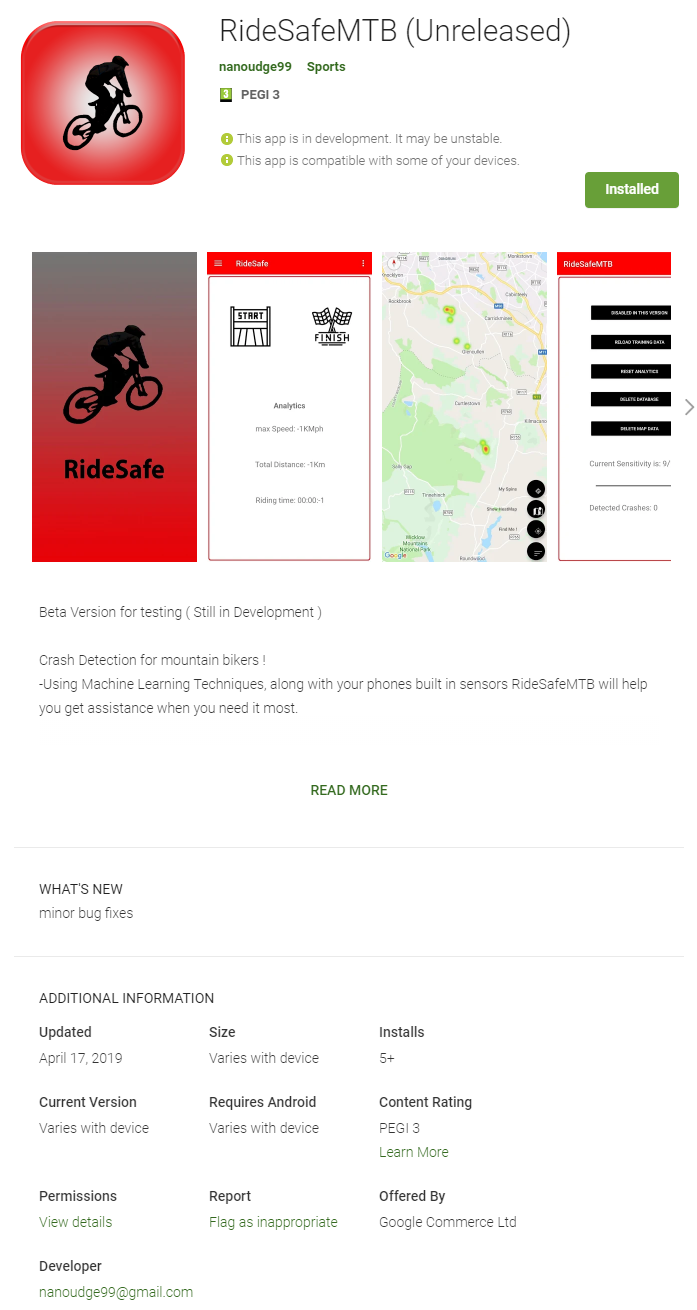
\includegraphics[scale = 1.3]{conclusion/Capture.png}
      \caption{Play Store Listing For RideSafe}
      \label{store}
\end{figure}
%%%%%%%%%%%%%%%%%%%%%%%%%%%%%%%%%%%%%%%%

\bibliographystyle{unsrtnat}
\bibliography{bibs/references}
\appendix
\renewcommand{\thechapter}{A\arabic{chapter}}
\chapter{Appendix}

\section{Other Resources}

A beta version of Ridesafe is currently availible on the Google Play store which can be accessed by folloing this link: https://play.google.com/store/apps/details?id=com.release.nanou.ridesafe

The source code for RideSafe is availible on the authors Github account : https://github.com/monganai/RideSafe


\section{Supplied With This Report}

Supplied with this report is a rescorce containing:

\begin{itemize}
\item The source code for RideSafe as well as a pre-compiled version of the application (.APK File)

\item A subset of collected sensor values used for analyzing and training RideSafe

\end {itemize}

\newpage

\section{Application Screenshots}


%%%%%%%%%%%%%%%%%%%%%%%%%%%%%%%%%%%%%%%%
\begin{figure}[h]
      \centering
      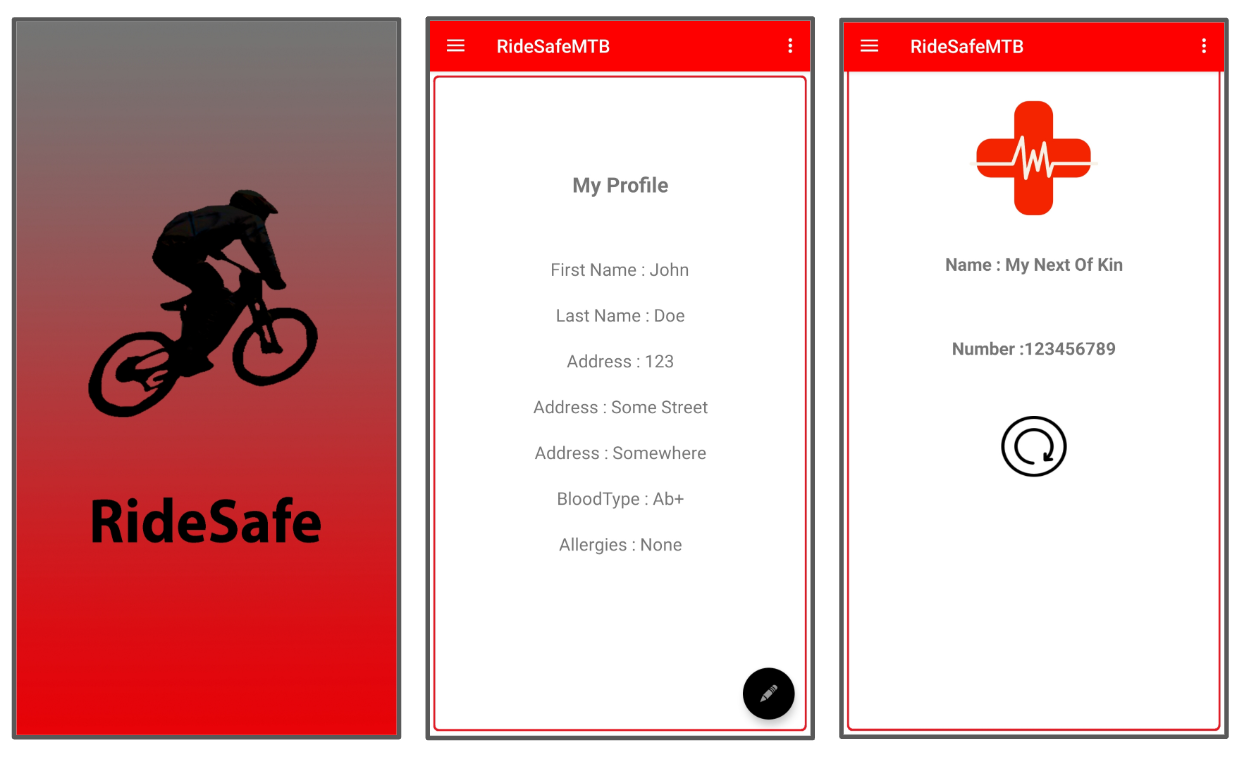
\includegraphics[scale = .9]{appendix/1.png}
      \caption{}
      \label{1}
\end{figure}
%%%%%%%%%%%%%%%%%%%%%%%%%%%%%%%%%%%%%%%%




%%%%%%%%%%%%%%%%%%%%%%%%%%%%%%%%%%%%%%%%
\begin{figure}[h]
      \centering
      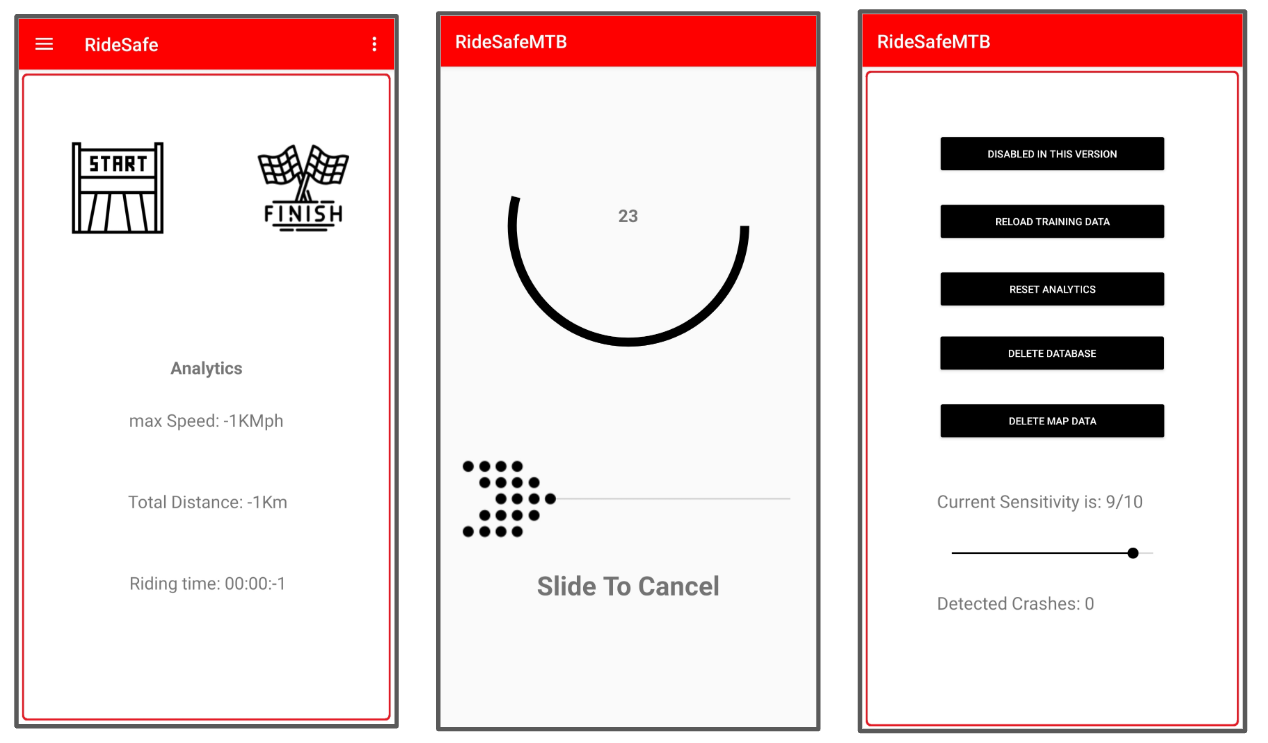
\includegraphics[scale = .9]{appendix/2.png}
      \caption{}
      \label{2}
\end{figure}
%%%%%%%%%%%%%%%%%%%%%%%%%%%%%%%%%%%%%%%%




%%%%%%%%%%%%%%%%%%%%%%%%%%%%%%%%%%%%%%%%
\begin{figure}[h]
      \centering
      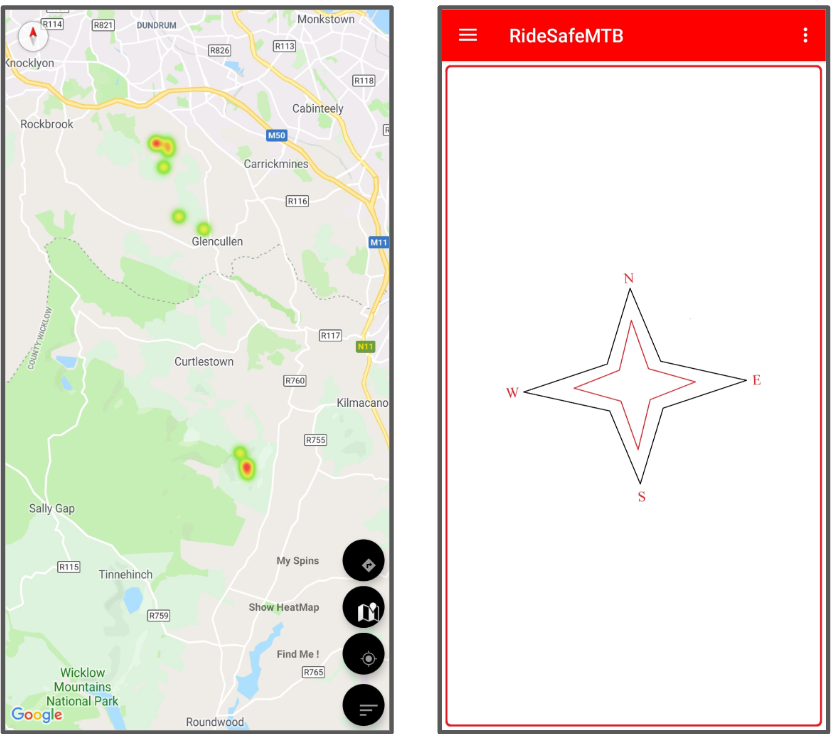
\includegraphics[scale = .9]{appendix/3.png}
      \caption{}
      \label{cm}
\end{figure}
%%%%%%%%%%%%%%%%%%%%%%%%%%%%%%%%%%%%%%%%



\end{document}